\documentclass[fr]{../../../eplsummary}

\usepackage[minted]{../../../eplcode}
\usepackage{float}
\usepackage{colonequals}
\usepackage[french,ruled,vlined]{algorithm2e}
\usepackage{csquotes}
\usepackage{footnote}
\usepackage{centernot}
\usepackage{colonequals}

\graphicspath{{img/}}

\newcommand{\prop}{\langle \textit{proposition} \rangle}
\newcommand{\form}{\langle \textit{formule} \rangle}
\newcommand{\prodop}{\ratio\:\!\ratio\:\!=}
\newcommand{\true}{\textnormal{true}}
\newcommand{\false}{\textnormal{false}}
\newcommand{\EP}{\mathcal{E}_P}
\newcommand{\val}[1]{\mathrm{val}_{#1}}
\newcommand{\VAL}[1]{\mathrm{VAL}_{#1}}
\newcommand{\tauto}{{\vDash} \>}
\newcommand{\contra}{{\nvDash} \>}
\providecommand{\lxor}{\oplus}
\newcommand{\logcons}{\Rrightarrow}
\newcommand{\logeq}{\mathrel{\Lleftarrow {} \mspace{-12mu} {} \Rrightarrow}}
\newcommand{\nimplies}{\centernot\implies}
\newcommand{\soom}{\sim}
\newcommand{\hub}{\mathrm{hub}}
\newcommand{\auth}{\mathrm{auth}}
\newcommand{\PR}{\mathrm{PR}}

\SetKwComment{Comment}{$\triangleright$\ }{}

% TODO rewrite bnf grammar with syntax package (didn't work for me :^( )
% TODO add some figures perhaps

\hypertitle{Logique et structures discrètes}{5}{INGI}{1101}
{Gilles Peiffer}
{Peter Van Roy}

\part{Logique}
\section{Contexte: la méthode scientifique}
La logique est la science du raisonnement.
Il existe 3 types de raisonnement:
\begin{itemize}
	\item la déduction\footnote{Qu'on étudiera dans ce cours.};
	\item l'induction;
	\item l'abduction.
\end{itemize}
Tout raisonnement fait par un humain
fait partie de l'une de ces trois catégories.
Prenons l'exemple de la méthode scientifique.
L'humain commence en général par émettre une théorie
sur comment fonctionne le monde,
et ce en se basant sur un modèle théorique du monde réel.
Ensuite, à partir de cette théorie,
il est possible de \emph{déduire} les résultats
que devrait avoir une certaine expérience,
si la théorie est juste.
On effectue alors l'expérience,
et on \emph{induit} à partir des résultats
une règle que semble suivre la nature.
Finalement, observant cette règle naturelle,
on la compare avec la théorie proposée,
et si les deux ne sont pas en accord,
on se pose la question \foreignquote{french}{Pourquoi la nature suit-elle cette règle?}.
La réponse à cette question est une abduction.
\begin{figure}[H]
	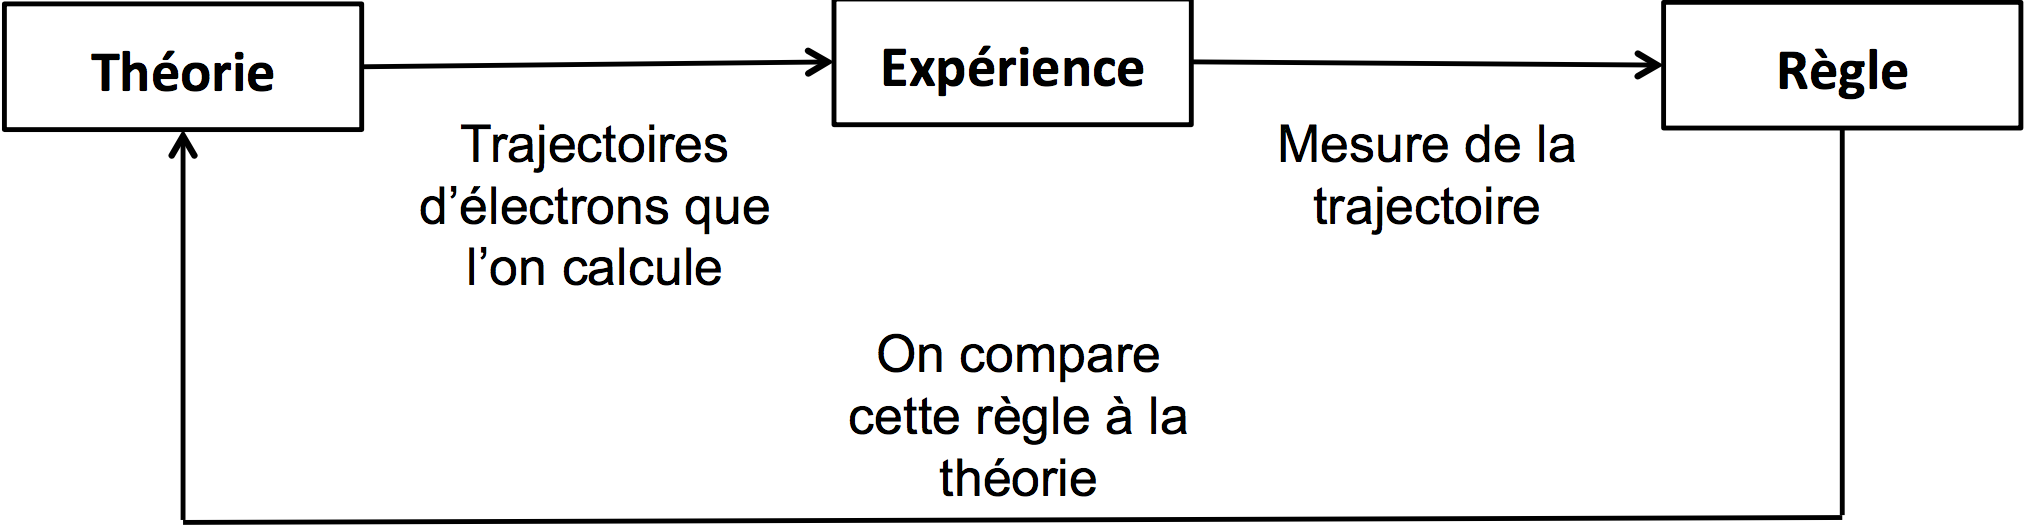
\includegraphics[width=\textwidth]{scientific_method}
	\caption{Un exemple d'utilisation de la méthode scientifique
	pour les lois de Maxwell.
	Notons que ce schéma n'est pas entièrement complet:
	il faudrait séparer la partie \foreignquote{french}{Expérience} en deux;
	d'une part tout ce qui est prédiction,
	et d'autre part la mise en place.
	La théorie permet alors de faire les deux.}
	\label{fig:sci_meth}
\end{figure}
\bigbreak
On remarque donc que sur ces trois raisonnements,
uniquement la déduction est un raisonnement sûr,
alors que l'induction et l'abduction ne le sont pas.
\begin{myexem}[Sac de billes]
Un exemple illustrant cette différence
serait un sac rempli de billes colorées.
On suppose que la théorie nous dit
que toutes les billes sont blanches.
On \emph{déduit} donc avec parfaite sûreté
que si on pioche une bille du sac,
elle sera blanche.

Comparons cela avec le cas suivant:
on est en train de piocher des billes du sac,
et on remarque que toutes les billes que l'on pioche sont blanches.
On peut alors \emph{induire} que toutes les billes du sac sont blanches.
Ce raisonnement n'est pas parfaitement sûr,
contrairement à la déduction.

Finalement, supposons que l'on trouve un bille blanche à coté du sac.
On pourrait expliquer cela par le fait que les billes viennent du sac.
Il s'agit d'un raisonnement abductif,
qui n'est d'ailleurs pas sûr.
\end{myexem}

\section{La logique propositionnelle}
La logique propositionnelle
est la plus simple des formes de logique
(on a également la logique des prédicats\footnote{Plus tard dans le cours\dots},
la logique du second ordre, la logique temporelle, la logique modale,\dots).
Elle permet de formaliser les connexions logiques entre des propositions.
\bigbreak
\begin{mydef}[Proposition première]
	Les \emph{propositions premières} sont les \foreignquote{french}{briques}
	avec lesquelles nous construisons les propositions plus compliquées.
	Elles peuvent soit être vraies (true) ou fausses (false).
	Un exemple pourrait être la phrase
	\foreignquote{french}{La logique est compliquée.}\footnote{En l'occurrence, cette proposition est fausse\dots}.
	On les dénote avec des lettres majuscules ($A$, $B$,\dots).
\end{mydef}
\begin{mydef}[Proposition logique]
	Une \emph{proposition logique} est alors soit une proposition première,
	soit une combinaison de propositions logiques
	connectées par des connecteurs logiques.
\end{mydef}
L'avantage de cette notation est qu'elle permet de raisonner formellement
sur les propositions logiques.
On peut définir:
\begin{enumerate}
	\item une \emph{syntaxe} (définie par une grammaire)
	qui définit ce qui est une proposition logique et ce qui ne l'est pas;
	\item une \emph{sémantique}
	qui donne un sens à chaque proposition logique;
	\item une \emph{théorie de preuve} permettant,
	en sachant qu'une proposition est vraie,
	de trouver d'autres propositions vraies.
\end{enumerate}
\subsection{Syntaxe}
\label{sec:syntax}
La logique propositionnelle est un \emph{langage formel}.
Ce langage peut être défini à l'aide d'une grammaire sur un \emph{alphabet}.
Cet alphabet est l'ensemble des symboles qui composent une proposition logique:
\begin{itemize}
	\item les lettres majuscules pour les propositions premières: $A$, $B$,\dots;
	\item $\true$ et $\false$ pour les propositions
	resp. toujours vraie et toujours fausse;
	\item les caractères de ponctuation: $($ et $)$;
	\item les connecteurs logiques:
	\begin{itemize}
		\item la conjonction (\textsc{and}): $\land$;
		\item la disjonction (\textsc{or}): $\lor$;
		\item la négation (\textsc{not}): $\lnot$;
		\item l'implication: $\to$ ou $\implies$;
		\item l'équivalence: $\leftrightarrow$ ou $\iff$.
	\end{itemize}
	Leur précédence est la suivante:
	\begin{table}[H]
		\[
		\begin{array}{cc}
			\hline
			\textnormal{Connecteur} & \textnormal{Précédence}\\
			\lnot & 1\\
			\land & 2\\
			\lor & 3\\
			\to & 4\\
			\leftrightarrow & 5\\
			\hline
		\end{array}
		\]
	\end{table}
\end{itemize}
La grammaire suivante permet de donner les règles
que doivent respecter les phrases propositionnelles:
\[
\renewcommand{\arraystretch}{1.5}
\begin{array}{rrl}
	\langle \textit{identificateur} \rangle & \prodop & A \mid B \mid C \mid \dots\\
	\prop &\prodop& \true\\
	&\mid& \false\\
	&\mid& \langle \textit{identificateur} \rangle\\
	&\mid& \big(\prop\big)\\
	&\mid& \lnot \prop\\
	&\mid& \prop \land \prop\\
	&\mid& \prop \lor \prop\\
	&\mid& \prop \to \prop\\
	&\mid& \prop \leftrightarrow \prop
\end{array}
\]

On remarque qu'uniquement les séquences de symboles
qui respectent cette grammaire
sont des phrases propositionnelles.
\paragraph{Métalangage}
Le métalangage est un deuxième langage utilisé pour parler d'un premier,
dans notre cas, la logique propositionnelle.
Notre métalangage est le français,
auquel on ajoute les notations mathématiques.
Ce concept est important pour distinguer raisonnement formel et informel.
\subsection{Tables de vérité}
La syntaxe développée à la \sectionref{syntax}
permet d'écrire les propositions en logique formelle,
mais ne leur donne pas de sens (vrai ou faux).
Afin de donner un sens aux propositions,
il faut commencer par déterminer
si les propositions premières sont vraies ou fausses.
Pour cela, il y a deux approches:
les \emph{tables de vérité}
et les \emph{interprétations}.
Les propositions logiques sont construites
à partir de propositions plus simples.
Une table de vérité est une façon de partir
des valeurs de différentes propositions
pour déterminer la valeur d'une autre proposition.
Voici les tables de vérité des différents connecteurs logiques
(le connecteur XOR ($p \lxor q$)
est une façon plus simple
d'écrire $\lnot(p \land q) \land (p \lor q)$):
\begin{table}[H]
	\[
	\begin{array}{cc|c|c|c|c|c|c}
		p & q & p \land q & p \lor q & \lnot p & p \to q & p \leftrightarrow q & p \lxor q\\
		\hline
		\true & \true & \true & \true & \multirow{2}{*}{\false} & \true & \true & \false\\
		\true & \false & \false & \true & & \false & \false & \true \\
		\false & \true & \false & \true & \multirow{2}{*}{\true} & \true & \false & \true\\
		\false & \false & \false & \false & & \true & \true & \false
	\end{array}
	\]
\end{table}
\subsection{Interprétations}
On peut également définir si une proposition est vraie ou fausse
en utilisant une \emph{interprétation}.
Soit $\EP$ l'ensemble des propositions premières.
Alors, une interprétation $I$ définit
une fonction de valuation $\val{I} \colon \EP \to \{\,\true,\false\,\}$,
qui permet de savoir si ces propositions premières sont vraies ou fausses\footnote{La notation $f \colon \mathcal{A} \to \mathcal{B}$
signifie ici que $f$ est une fonction
depuis l'ensemble $\mathcal{A}$ vers l'ensemble $\mathcal{B}$.}.
On pourrait par exemple écrire
\begin{align*}
	\left\{
	\begin{array}{rcl}
		\val{I_1}(P) & = & \true\,,\\
		\val{I_1}(Q) & = & \false
	\end{array}
	\right.
	\quad \textnormal{et} \quad
	\left\{
	\begin{array}{rcl}
		\val{I_2}(P) & = & \true\,,\\
		\val{I_2}(Q) & = & \true\,.
	\end{array}
	\right.
\end{align*}
Il y a donc différentes interprétations possibles,
et chacune d'elles risque de donner un résultat différent.
\bigbreak
À partir de ces fonctions de valuation premières,
on peut définir d'autres fonctions de valuation:
$\VAL{I}$ se définit par rapport à $\val{I}$.
On a ainsi
\begin{align*}
	\VAL{I}(P) &= \val{I}(P)\,,\quad \forall P \in \EP\,,\\
	\VAL{I}(\lnot P) &=
	\left\{
	\begin{array}{l}
		\false \textnormal{ si } \VAL{I}(P) = \true\,,\\
		\true \textnormal{ sinon}\,,
	\end{array}
	\right.\\
	\VAL{I}(P \land Q) &=
	\left\{
	\begin{array}{l}
		\true \textnormal{ si } \VAL{I}(P) = \true \textnormal{ et } \VAL{I}(Q) = \true\,,\\
		\false \textnormal{ sinon}\,,
	\end{array}
	\right.\\
	\VAL{I}(P \lor Q) &=
	\left\{
	\begin{array}{l}
		\true \textnormal{ si } \VAL{I}(P) = \true \textnormal{ ou } \VAL{I}(Q) = \true\,,\\
		\false \textnormal{ sinon}\,.
	\end{array}
	\right.
\end{align*}
\subsection{Les modèles logiques}
Une interprétation est un modèle $M$ pour une certaine théorie si
les propositions premières sont telles
que tous les axiomes de la théorie soient vrais.
\begin{myexem}
	Prenons le cas suivant:
	\begin{align*}
		&L\textnormal{: \foreignquote{french}{Le cours de logique est facile.},}\\
		&E\textnormal{: \foreignquote{french}{L'étudiant a bien étudié.},}\\
		&R\textnormal{: \foreignquote{french}{L'étudiant a réussi l'examen de logique.},}
	\end{align*}
	\[
	\big(L \land E\big) \to R\,.\tag*{Axiome~(1)}
	\]
	Un modèle possible des études supérieures serait donc
	\[
	(L,E,R) = (\true,\true,\true)\,.
	\]
\end{myexem}
On peut donc dire que la théorie est un ensemble de formules
et que le modèle est une interprétation qui satisfait ces formules.
\bigbreak
Soit une formule $p$ aléatoire.
\begin{mydef}[Tautologie]
	Si $p$ est vraie dans toutes les interprétations possibles,
	alors on dit que $p$ est une tautologie ($\tauto p$).
	On a par exemple $p \equiv \big(P \lor \lnot P\big)$.
\end{mydef}
\begin{mydef}[Contradiction]
	Si $p$ est fausse dans toutes les interprétations possibles,
	alors on dit que $p$ est une contradiction ($\contra p$).
	On a par exemple $p \equiv \big(P \land \lnot P\big)$.
\end{mydef}
\begin{mydef}[Contingence]
	Si $p$ n'est ni une tautologie,
	ni une contradiction,
	on dit que $p$ est contingente.
	Par exemple, $p \equiv \big(P \land \lnot Q\big)$.
\end{mydef}
\subsubsection{Conséquence logique}
On note \foreignquote{french}{$q$ est conséquence logique de $p$}
par $p \logcons q$\footnote{Le Prof. Van Roy
utilise les notations $p \logcons q$ et $p \logeq q$
pour la conséquence et l'équivalence logique.
Cependant, dans la littérature,
on utilise $p \implies q$ et $p \iff q$ pour celles-ci.
Comme le Prof. Van Roy utilise déjà celles-ci
pour la conséquence et l'équivalence matérielles
(qui dans la littérature sont souvent représentées
par $p \to q$ et $p \leftrightarrow q$),
on reprendra donc sa notation,
bien qu'elle soit non standard.}.
Soit $p \vDash q$.
Cela veut dire que si $M$ est modèle de $p$, alors $M$ est aussi modèle de $q$.
On a donc $\tauto (p \to q)$,
car $p \to q$ est toujours vrai.
On peut donc bien écrire $p \logcons q$.
\begin{myexem}
	Soit $p \equiv \big(P \land Q\big)$ et $q \equiv \big(P\big)$.
	On a alors que $p \vDash q$.
\end{myexem}
La conséquence logique $p \logcons q$ fait partie du métalangage,
et n'est donc pas une proposition logique.
\subsubsection{Équivalence logique}
Par un raisonnement similaire,
si on a $p \vDash q$ et $q \vDash p$,
on a également $\tauto (p \to q)$ et $\tauto (q \to p)$.
On peut donc écrire $p \logeq q$.
L'équivalence logique n'est pas non plus une proposition logique
mais fait partie du métalangage.

\section{Preuves en logique propositionnelle}
\begin{mydef}[Preuve]
	Une \emph{preuve} est un raisonnement déductif
	qui démontre si une proposition est vraie ou fausse.
	On distingue les preuves \emph{formelles} et \emph{informelles}.
	\begin{itemize}
		\item Une \emph{preuve formelle}
		est un raisonnement en langage naturel,
		parfois augmenté avec des notations mathématiques.
		\item Une \emph{preuve informelle}
		est un raisonnement mathématique
		qui formalise le raisonnement déductif.
	\end{itemize}
\end{mydef}
\begin{myrem}
	\foreignquote{french}{On peut prouver $q$ à partir de $p$} se note $p \vdash q$.
\end{myrem}
\subsection{Preuve avec table de vérité}
La preuve formelle la plus simple est une table de vérité.
On fait un tableau avec $2^n$ lignes,
où $n$ est le nombre de propositions premières,
et pour chaque ligne,
on prouve une équivalence.
Cette méthode de preuve a l'inconvénient d'être très longue,
et en pratique elle n'est pas réellement utile
au-delà d'une centaine de propositions premières.
On appelle ces programmes (qui ont des heuristiques supplémentaires)
des \textsc{sat} solvers.
Elle n'est également pas valable pour la logique des prédicats.
\subsection{Preuve transformationnelle}
Une preuve transformationnelle est une séquence de transformations
\[
p_1 \logeq p_2 \logeq \cdots \logeq p_n
\]
dans laquelle on a toujours $p_i \logeq p_{i+1}$.
Une preuve transformationnelle est aussi un objet mathématique en métalangage.
On utilise pour ceci des \foreignquote{french}{lois} de transformation,
c'est-à-dire des équivalences connues.
\begin{table}[H]
\renewcommand\arraystretch{1.5}
\centering
\begin{tabular}{rcl@{\qquad}l}
	\hline
	$p$ & $\logeq$ & $p \lor p$ & Idempotence de $\lor$ \\
	$p$ & $\logeq$ & $p \land p$ & Idempotence de $\land$ \\
	$p \lor q$ & $\logeq$ & $q \lor p$ & Commutativité de $\lor$ \\
	$p \land q$ & $\logeq$ & $q \land p$ & Commutativité de $\land$ \\
	$(p \lor q) \lor v$ & $\logeq$ & $p \lor (q \lor v)$ & Associativité de $\lor$ \\
	$(p \land q) \land v$ & $\logeq$ & $p \land (q \land v)$ & Associativité de $\land$ \\
	$\lnot \lnot p$ & $\logeq$ & $p$ & Double négation \\
	$p \to q$ & $\logeq$ & $\lnot p \lor q$ & Implication \\
	$\lnot(p \land q)$ & $\logeq$ & $\lnot p \lor \lnot q$ & 1\ieme{} loi de De Morgan \\
	$\lnot(p \lor q)$ & $\logeq$ & $\lnot p \land \lnot q$ & 2\ieme{} loi de De Morgan \\
	$p \leftrightarrow q$ & $\logeq$ & $(p \to q) \land (q \to p)$ & Équivalence \\
	$(p \land q) \lor r$ & $\logeq$ & $(p \lor r) \land (q \lor r)$ & Distributivité de $\lor$ \\
	$(p \lor q) \land r$ & $\logeq$ & $(p \land r) \lor (q \land r)$ & Distributivité de $\land$ \\
	\hline
\end{tabular}
\caption{Lois de transformation.}
\label{tab:trans}
\end{table}
Pour réellement utiliser ces lois,
on rajoute deux lois supplémentaires:
\begin{itemize}
	\item La \emph{transitivité de l'équivalence}.

	Si $p \logeq q$ et $q \logeq r$,
	alors $p \logeq r$.
	\item Le \emph{principe de substitution}.

	On peut remplacer une sous-formule
	par une autre sous-formule équivalente
	à l'intérieur d'une formule.
\end{itemize}

\subsection{Preuve déductive}
Une preuve déductive est un objet mathématique
qui formalise une séquence de pas de raisonnement simples.
Chaque pas doit être justifié
avec le nom de la règle ou la loi qui est utilisée.
Les pas utilisent trois techniques de raisonnement différentes:
les équivalences logiques,
les règles d’inférence et
les schémas de preuve.
\subsubsection{Équivalences logiques}
Les équivalences logiques sont les mêmes
que celles données dans la \tabref{trans}.
\subsubsection{Règles d'inférence}
Contrairement aux preuves transformationnelles, les règles d'inférence
ont une direction:
elles commencent par les prémisses et terminent par une conclusion.
On utilise un raisonnement informel pour justifier les règles.

\begin{table}[H]
\centering
\renewcommand{\arraystretch}{1.5}
\begin{tabular}{cl@{\qquad\qquad}cl}
	\hline
	$\begin{array}{c}
	p \\
	q \\
	\hline
	p \land q
	\end{array}$ & Conjonction & $\begin{array}{c}
	p \\
	\lnot p \\
	\hline
	q
	\end{array}$ & Contradiction \\
	&&&\\
	$\begin{array}{c}
	p \land q \\
	\hline
	p
	\end{array}$ & Simplification & $\begin{array}{c}
	p \\
	\hline
	p \lor q
	\end{array}$ & Addition \\
	&&&\\
	$\begin{array}{c}
	p \leftrightarrow q\\
	q \leftrightarrow r\\
	\hline
	p \leftrightarrow r
	\end{array}$ & Transitivité de l'équivalence & $\begin{array}{c}
	p \lor q\\
	\lnot p \\
	\hline
	q
	\end{array}$ & Syllogisme disjoint \\
	&&&\\
	$\begin{array}{c}
	p \to q \\
	p \\
	\hline
	q
	\end{array}$ & Modus ponens & $\begin{array}{c}
	p \to q \\
	\lnot q \\
	\hline
	\lnot p
	\end{array}$ & Modus tollens \\
	&&&\\
	$\begin{array}{c}
	p \leftrightarrow q \\
	\hline
	q \leftrightarrow p
	\end{array}$ & Loi d'équivalence & $\begin{array}{c}
	\lnot \lnot p \\
	\hline
	p
	\end{array}$ & Double négation \\
	\hline
\end{tabular}
\caption{Ensemble des règles d'inférence utilisées.}
\label{tab:inference}
\end{table}

\subsubsection{Schémas de preuve}
En plus des équivalences logiques et des règles d'inférence,
on a deux schémas de preuve
qui formalisent des techniques de raisonnement plus abstraites:
le théorème de déduction et la démonstration par l'absurde.
En général, on met ces preuves dans des schémas comme celui en \figuref{proof}.
\begin{figure}[H]
\centering
\begin{tabular}{ccc}
	& Formule & Justification \\
	\hline
	1. & $s$ & $\cdots$ \\
	2. & $\cdots$ & $\cdots$ \\
	\multirow{3}{*}{$\vdots$} & \multirow{3}{*}{$\vdots$} & \multirow{3}{*}{$\vdots$} \\
	&&\\
	&&\\
	$n$. & $t$ & $\cdots$\\
	\hline
\end{tabular}
\caption{Le squelette d'une preuve en logique propositionnelle.}
\label{fig:proof}
\end{figure}
\paragraph{Théorème de déduction (preuve conditionnelle)}
Supposons $s$ vraie.
C'est notre hypothèse.
Elle s'ajoute donc aux prémisses utilisées dans la preuve.
Ensuite, on fait une preuve de $t$.
On peut construire une preuve (objet mathématique) de $t$ en commençant de $s$.
On note ceci $s \vdash t$.
\[
\begin{array}{lcr}
	p,\dots,r,s & \vdash & t \\
	\hline
	p,\dots,r & \vdash & s \to t
\end{array}
\]
On a évacué l'hypothèse.
\paragraph{Démonstration par l'absurde (preuve par contradiction)}
Également appelée \emph{reductio ad absurdum}.
On suppose nos prémisses $p,\dots,q$ sans contradiction.
On rajoute $r$ aux prémisses.
Si on peut prouver $s$ et $\lnot s$,
cela signifie que $r$ rend les prémisses inconsistantes.
\[
\begin{array}{lcr}
	p,\dots,q,r & \vdash & s \\
	p,\dots,q,r & \vdash & \lnot s\\
	\hline
	p,\dots,q & \vdash & \lnot r
\end{array}
\]
\subsection{Algorithme de preuve}
Les preuves manuelles de la section précédente
ont un grand défaut:
elles sont extrêmement lentes.
Afin de diminuer le temps nécessaire pour prouver une équivalence logique,
on peut définir un algorithme de preuve,
qui est une automatisation d'une démonstration par l'absurde
qui est basée sur une seule règle,
la \emph{résolution}.

\subsubsection{Transformation en forme normale conjonctive}

Toute formule logique peut être transformée en une formule équivalente,
qui est une conjonction de disjonctions.
C'est la forme normale conjonctive (\textsc{fnc}).
On peut également définir une forme similaire,
la \textsc{fnd} (forme normale disjonctive),
qui est donc une disjonction de conjonctions.

\paragraph{Terminologie}
Afin de faciliter la discussion autour des formes normales,
on introduit la terminologie suivante:
\begin{itemize}
	\item Un \emph{littéral} $L$ est soit une proposition première,
	soit la négation d'une proposition première.
	\item Une \emph{clause} $C$, en \textsc{fnc},
	est une disjonction de littéraux.
	On écrit
	\begin{align*}
	C &\equiv \bigvee\limits_{i = 1}^{n} L_i\\
	&\equiv L_1 \lor L_2 \lor \dots \lor L_n\,.
	\end{align*}
	En \textsc{fnc}, on a souvent des conjonctions de clauses,
	c'est-à-dire des formules de la forme
	\begin{align*}
	\bigwedge\limits_{i=1}^{m} C_i &\equiv \bigwedge\limits_{i = 1}^{m} \bigvee\limits_{j = 1}^{n_i} L_{ij}\\
	&\equiv \big(L_{11} \lor \dots \lor L_{1n_1}\big) \land \dots \land \big(L_{m1} \lor \dots \lor L_{mn_m}\big) \,.
	\end{align*}
\end{itemize}

\paragraph{Algorithme de normalisation}
Pour mettre sous \textsc{fnc} une formule logique quelconque,
on utilise l'algorithme suivant:
\begin{enumerate}
	\item éliminer les implications et équivalences matérielles
	($\to$ et $\leftrightarrow$)
	en les remplaçant par des formules équivalentes;
	\item déplacer les négations vers l'intérieur
	(jusqu'aux propositions premières)
	en utilisant les formules de De Morgan;
	\item déplacer les disjonctions ($\lor$) vers l'intérieur
	en utilisant les lois distributives;
	\item simplifier en éliminant les formes $(P \lor \lnot P)$
	dans chaque disjonction.
\end{enumerate}

\subsubsection{Résolution}
La règle de résolution est l'unique règle d'inférence utilisée
dans les algorithmes de preuve.
Elle s'écrit comme suit:
\[
\begin{array}{l@{}c@{}r}
	p_1 & {} \lor {} & q\\
	p_2 & {} \lor {} & \lnot q\\
	\hline
	p_1 & {} \lor {} & p_2
\end{array}
\]
\begin{myrem}[La résolution préserve les modèles]
\end{myrem}
\begin{proof}
	Soient
	\begin{align*}
		p &\equiv \bigwedge\limits_{i=1}^{2} C_i\,,\\
		C_1 &\equiv p_1 \lor q\,,\\
		C_2 &\equiv p_2 \lor \lnot q\,,\\
		r &\equiv p_1 \lor p_2\\
		&\equiv \left(C_1 - \{\,P\,\}\right) \lor \left(C_2 - \{\,\lnot P\,\}\right)\,.
	\end{align*}
	$r$ est une nouvelle disjonction à partir de deux autres disjonctions.
	Prouvons que $r$ est toujours vraie ($\{\,C_1, C_2\,\} \vDash r$).
	On utilise pour cela la sémantique,
	une preuve en métalangage qui n'est donc pas formalisée.

	Si
	\[
	\left\{
	\begin{array}{c}
		\VAL{I}(C_1) = \true\,,\\
		\VAL{I}(C_2) = \true\,,
	\end{array}
	\right.
	\]
	alors $I$ est modèle de $\{\,C_1, C_2\,\}$.

	On voit que c'est le cas,
	car on a toujours soit $\VAL{I}(q) = \true$
	et donc $\VAL{I}(p_2) = \true$,
	ou bien $\VAL{I}(q) = \false$
	et donc $\VAL{I}(p_1) = \true$.
	$r$ est donc toujours vraie.
\end{proof}

\subsubsection{Pseudocode}

Prenons des axiomes $C_i$ en \textsc{fnc}:
\begin{align*}
C_i &= \bigvee\limits_{i=1}^{n} L_i\,,\\
L_i &= P \textnormal{ ou } \lnot P\,,
\end{align*}
et un théorème à prouver, $C$.
On veut donc démontrer
\[
\{\,C_1, \dots,C_n\,\} \vdash C\,.
\]
On sait que
\[
\{\,C_1, \dots, C_n\,\} \vDash C \iff \{\,C_1, \dots, C_n, \lnot C\,\} \vDash \false\,.
\]
Il suffit donc de démontrer que $\mathcal{S} = \{\,C_1, \dots, C_n, \lnot C\,\}$
est inconsistant.
Pour faire cela,
l'algorithme de preuve combine les éléments de $\mathcal{S}$
grâce à la résolution,
jusqu'à ce qu'on arrive à une contradiction,
ou qu'il n'y ait plus de possibilité d'utiliser la résolution.
Dans le premier cas,
nous avons prouvé $C$.
Dans le second,
$C$ est improuvable.

\begin{algorithm}[H]
\DontPrintSemicolon
\KwData{$C_1,\dots,C_n$ les clauses, et $C$ le théorème à prouver.}
\KwResult{Si oui ou non $C_1, \dots, C_n \vdash C$.}
\Begin{
	$\mathcal{S} \gets \{\,C_1, \dots, C_n, \lnot C\,\}$\;
	\While{$\false \notin \mathcal{S}$ et
	$\exists C_i, C_j \in \mathcal{S}$ telles que $C_i, C_j$
	résolvables et non résolues}{
		choisir $C_1, C_2 \in \mathcal{S}$
		telles que $\exists P \in C_1, \lnot P \in C_2$\;
		calculer $r \gets C_1 \setminus \{\,P\,\} \lor C_2 \setminus \{\,\lnot P\,\}$\;
		calculer $\mathcal{S} \gets \mathcal{S} \cup \{\,r\,\}$\;
	}
	\eIf{$\false \in \mathcal{S}$}{
		\Return \true \Comment*[r]{$C$ prouvé}
	}{
		\Return \false \Comment*[r]{$C$ improuvable}
	}
}
\caption{Algorithme de preuve\label{algo:proof}}
\end{algorithm}

En plus de prouver l'existence éventuelle d'une preuve,
l'algorithme de preuve nous donne également cette preuve.

\begin{myprop}[Propriétés de l'algorithme de preuve en logique propositionnelle]
	Pour toute théorie $\mathcal{B} = \{\,C_1, \dots, C_n\,\}$ et théorème $C$,
	l'algorithme de preuve est
	\begin{itemize}
		\item \textbf{Décidable (\emph{decidable}).}
		L'algorithme se termine
		après un nombre fini d'étapes $\forall \mathcal{B}, C$.
		\item \textbf{Adéquat (\emph{sound}).}
		Si $\mathcal{B} \vdash C$,
		alors $\mathcal{B} \vDash C$.
		\item \textbf{Complet (\emph{complete}).}
		Si $\mathcal{B} \vDash C$,
		alors $\mathcal{B} \vdash C$.
	\end{itemize}

	Le temps d'exécution
	est exponentiel en le nombre de propositions premières
	et de clauses\footnote{Bien que ce temps d'exécution
	puisse être fortement amélioré
	par l'utilisation de diverses heuristiques,
	comme celles utilisées dans les \textsc{sat} solvers.}.
\end{myprop}

\section{La logique des prédicats}
Étudions maintenant une logique plus expressive,
la logique des prédicats ou logique de premier ordre.
Les principales différences avec la logique propositionnelle sont:
\begin{itemize}
	\item Les propositions premières sont remplacées
	par des prédicats.
	\item On introduit les quantificateurs existentiel et universel.
	\item Il est possible d'exprimer
	des relations entre les éléments d'un ensemble de façon concise,
	même lorsque cet ensemble est de taille infinie.
\end{itemize}

\subsection{Quantificateurs}
Afin de noter clairement
le fait de dire \foreignquote{french}{pour tout $x$} et
\foreignquote{french}{il existe un $x$ tel que},
on introduit la notion de quantificateur,
respectivement $\forall x$ et $\exists x$ dans ce cas-ci.
La \emph{portée} d'un quantificateur est la partie d'une phrase logique
dans laquelle il est d'application\footnote{En pratique, les quantificateurs sont suivis d'une variable, puis souvent d'un point.
Cette notation est due à Russell, Whitehead et Church et signifie que la portée de ce quantificateur va du point jusqu'à la fin de la phrase logique.}.
Afin de résoudre des conflits potentiels,
on fait appel à une nouvelle opération: le renommage des noms de variable.

\subsection{Syntaxe}
\subsubsection{Symboles}
Une formule en logique des prédicats peut utiliser différents symboles.
\begin{mydef}[Arité d'un prédicat]
	On appelle \foreignquote{french}{\emph{arité}} d'un prédicat
	(ou d'une fonction) le nombre d'arguments de celui-ci.
\end{mydef}
Les symboles utilisés sont montrés dans la \tabref{symbols}.
\begin{table}[H]
	\centering
	\begin{tabular}{ccc}
		\hline
		\multirow{5}{*}{Symboles logiques} & Quantificateurs & $\exists$ et $\forall$ \\
		 & Connecteurs logiques & $\land$, $\lor$, $\lnot$, $\to$ et $\leftrightarrow$ \\
		 & Caractères de ponctuation & $($ et $)$ \\
		 & \multirow{2}{*}{Variables} & $x$, $y$, $z$,\ldots \\
		 & & $\true$ et $\false$ \\
		\multirow{3}{*}{Symboles non logiques} & Symboles de prédicat & $P$, $Q$, $R$,\ldots (avec arité $\ge 0$) \\
		 & Symboles de fonction & $f$, $g$, $h$,\ldots (avec arité $\ge 0$) \\
		 & Symboles de constante & $a$, $b$, $c$,\ldots (si arité $= 0$) \\
		\hline
	\end{tabular}
	\caption{Symboles utilisés en logique des prédicats.}
	\label{tab:symbols}
\end{table}

\subsubsection{Règles de grammaire}
Les règles de grammaire en logique des prédicats sont les suivantes:
\[
\renewcommand{\arraystretch}{1.5}
\begin{array}{rrl}
	\form &\prodop & \langle \textit{formule atomique} \rangle\\
	&\mid& \lnot \form\\
	&\mid& \form \langle \textit{connecteur} \rangle \form\\
	&\mid& \forall \langle \textit{var} \rangle.\ \form\\
	&\mid& \exists \langle \textit{var} \rangle.\ \form\\
	\langle \textit{formule atomique} \rangle &\prodop& \true \mid \false\\
	&\mid& \langle \textit{prédicat} \rangle \big(\langle \textit{terme} \ast \rangle\big)\\
	\langle \textit{terme} \rangle &\prodop& \langle \textit{constante} \rangle\\
	&\mid& \langle \textit{var} \rangle\\
	&\mid& \langle \textit{fonction} \rangle \big(\langle \textit{terme} \ast \rangle\big)\\
	\langle \textit{connecteur binaire} \rangle &\prodop& \land \mid \lor \mid \to \mid \leftrightarrow\\
\end{array}
\]

\subsection{Sémantique}
En logique des prédicats nous gardons
les notions de modèle et d'interprétation
déjà définies pour la logique propositionnelle.
Comme pour la logique propositionnelle,
une interprétation a une valeur dans l'ensemble $\{\,\true, \false\,\}$.
\subsubsection{Interprétation}
\begin{mydef}[Interprétation en logique des prédicats]
	Une \emph{interprétation} $I$ en logique des prédicats
	est une paire $I = (\mathcal{D}_I, \val{I})$,
	où $\mathcal{D}_I$ est un ensemble appelé
	\foreignquote{french}{\emph{domaine de discours}}
	et $\val{I}$ est une \emph{fonction de valuation}
	qui renvoie un élément de $\mathcal{D}_I$ pour chaque symbole.
	Pour chaque symbole $s$, on a alors
	\begin{itemize}
		\item si $s$ est un symbole de prédicat,
		$\val{I}(s) = P_I \colon \mathcal{D}_I^n \to \{\,\true, \false\,\}$, avec $n$ le nombre d'arguments de $P_I$;
		\item si $s$ est un symbole de fonction,
		$\val{I}(s) = f_I \colon \mathcal{D}_I^n \to \mathcal{D}_I$, avec $n$ le nombre d'arguments de $f_I$;
		\item si $s$ est une constante (fonction sans arguments),
		$\val{I}(s) = c \in \mathcal{D}_I$;
		\item si $s$ est une variable,
		$\val{I}(s) = x_I \in \mathcal{D}_I$.
	\end{itemize}
	\begin{myrem}
		On remarque deux choses:
		\begin{itemize}
			\item Chaque fonction et chaque prédicat
			correspondent à une vraie fonction ou à un vrai prédicat,
			alors que chaque constante et chaque variable
			correspondent à une constante
			dans le domaine de discours, $\mathcal{D}_I$.
			\item L'interprétation est un élément de $\mathcal{D}_I$
			autant pour les constantes que pour les variables,
			mais les variables peuvent s'utiliser dans les quantificateurs
			alors que les constantes non.
		\end{itemize}
	\end{myrem}
\end{mydef}

Ayant défini la fonction $\val{I}$ sur tous les symboles,
on peut maintenant définir une fonction $\VAL{I}$
sur les termes et les formules:
\[
\VAL{I} \colon \mathcal{T} \cup \mathcal{P} \to \mathcal{D}_I \cup \{\,true, \false\,\}\,,
\]
où $\mathcal{T}$ est l'ensemble des termes et
$\mathcal{P}$ est l'ensemble des formules.
Nous avons donc:
\begin{itemize}
	\item si $t$ est un terme, $\VAL{I} \colon t \mapsto \VAL{I}(t)$;
	\item si $p$ est une formule, $\VAL{I} \colon p \mapsto \VAL{I}(p)$.
\end{itemize}
On peut définir $\VAL{I}$ à partir de $\val{I}$ comme suit:
\begin{itemize}
	\item $\VAL{I}\big(P(t_1, \ldots, t_m)\big) = \big(\val{I}(P)\big)\big(\VAL{I}(t_1), \ldots, \VAL{I}(t_m)\big)$.
	\item $\VAL{I}(\forall x.\ p) = \true$
	si pour chaque $d \in \mathcal{D}_I$,
	$\VAL{\{\,x \leftarrow d\,\} \circ I}(p) = \true$,
	$\false$ sinon.
	En clair, $d$ est l'interprétation de $x$ dans la formule $p$.
	Si $p$ est vraie pour tout $d$ dans le domaine de discours,
	alors le quantificateur universel est vrai aussi.
	\item $\VAL{I}(\exists x.\ p) = \true$
	s'il existe un élément $d \in \mathcal{D}_I$
	tel que $\VAL{\{\,x \leftarrow d\,\} \circ I}(p) = \true$,
	$\false$ sinon.
	\item $\VAL{I}(p \land q) = \true$
	si $\VAL{I}(p) = \VAL{I}(q) = \true$,
	$\false$ sinon.
	\item $\VAL{I}(p \lor q) = \true$
	si $\VAL{I}(p) = \true$ ou $\VAL{I}(q) = \true$,
	$\false$ sinon.
	\item $\VAL{I}(\lnot p) = \true$
	si $\VAL{I}(p) = \false$,
	$\false$ sinon.
	\item $\VAL{I}(p \to q) = \true$
	si $\VAL{I}(\lnot p \lor q) = \true$,
	$\false$ sinon.
	\item $\VAL{I}(p \leftrightarrow q) = \true$
	si $\VAL{I}\big((p \to q) \land (q \to p)\big) = \true$,
	$\false$ sinon.
	\item $\VAL{I}(c) = \val{I}(c)$
	si $c$ est un symbole de constante.
	\item $\VAL{I}(x) = \val{I}(x)$
	si $x$ est un symbole de variable.
	\item $\VAL{I}\big(f(t_1, \ldots, t_n)\big) = \big(\val{I}(f)\big)\big(\VAL{I}(t_1), \ldots, \VAL{I}(t_n)\big)$
	si $f$ est un symbole de fonction.
	\item $\VAL{I}(\true) = \true$.
	\item $\VAL{I}(\false) = \false$.
\end{itemize}
Il est donc possible de décomposer la formule $p$ en ses symboles de base
de sorte à pouvoir calculer $\VAL{I}(p)$ à partir de $\val{I}$.
\begin{mydef}[Modèle en logique des prédicats]
	Un \emph{modèle} d'un ensemble de formules
	est une interprétation qui rend toutes les formules vraies.
	Formellement,
	si on a un ensemble de formules $\mathcal{B} = \{\,p_1, \ldots, p_n\,\}$,
	une interprétation $I$ pour $\mathcal{B}$ est modèle si et seulement si
	\[
	\VAL{I}(p_i) = \true\,, \quad \forall p_i \in \mathcal{B}\,.
	\]
\end{mydef}

\section{Preuves en logique des prédicats}
Afin de traiter les quantificateurs en logique des prédicats,
nous utilisons l'approche suivante:
\begin{enumerate}
	\item enlever les quantificateurs pour avoir des variables libres;
	\item raisonner sur l'intérieur;
	\item remettre les quantificateurs.
\end{enumerate}
Afin de faire cela, il faut rajouter quatre règles
par rapport aux preuves formelles en logique propositionnelle\footnote{Les autres règles de la logique propositionnelle
restent valables en logique des prédicats.}:
\begin{itemize}
	\item élimination du quantificateur universel;
	\item introduction du quantificateur universel;
	\item élimination du quantificateur existentiel;
	\item introduction du quantificateur existentiel;
\end{itemize}

\subsection{Règles en logique des prédicats}
Avant de donner les règles de déduction pour les quantificateurs,
définissons une manipulation symbolique importante
qui est utilisée dans ces règles: la \emph{substitution}.

\begin{myrem}
	Il est impossible de prouver en logique des prédicats
	que les règles sont exactes.
	Chaque règle est justifiée par un raisonnement en métalangage,
	basée sur le modèle de la formule.
\end{myrem}

\subsubsection{Substitution}
La \emph{substitution} en logique des prédicats
consiste à prendre une formule et remplacer une partie par une autre.
\begin{mynota}[Substitution]
	Soit $p$ une formule quelconque; la notation $p[x/t]$ signifie
	que l'on remplace chaque occurrence libre de $x$ par $t$.
	\begin{mydef}[Occurrence libre]
		Une \emph{occurrence libre} d'une variable
		est une occurrence
		qui n'est pas dans la portée d'un quantificateur.
		Afin d'éviter la capture de variable,
		il faut faire un renommage des variables.
	\end{mydef}
\end{mynota}

\subsubsection{Élimination du quantificateur universel}
Comme $\forall x.\ P(x)$ veut dire
\foreignquote{french}{pour tout $x_I$ appartenant au domaine de discours,
$P_I(x_I)$ est vrai}, on peut remplacer sans contrainte:
\begin{align*}
\forall x.\ P(x) &\implies P(a)\,, \quad \textnormal{où $a$ est une constante quelconque,}\\
&\implies P(y)\,, \quad \textnormal{où $y$ est une variable (parce que $P_I(y_I)$ est vrai).}
\end{align*}
La règle s'écrit alors $\begin{array}{c}
	\forall x.\ p \\
	\hline
	p[x/t]
\end{array}$. Il est important de penser au renommage,
s'il est nécessaire.

\subsubsection{Introduction du quantificateur universel}
La règle s'écrit $\begin{array}{c}
	p \\
	\hline
	\forall x.\ p
\end{array}$.
On distingue plusieurs cas:
\begin{itemize}
	\item Si $p$ n'a pas d'occurrence libre de $x$, on peut le faire.
	\item Si $p$ contient une occurrence libre de $x$,
	on doit s'assurer que la preuve jusqu'à cet endroit
	fonctionne pour toutes les valeurs de $x$.
	Il ne peut donc pas y avoir de contraintes sur $x$ jusque là.
	Cela impose deux conditions:
	\begin{itemize}
		\item $x$ n'était pas libre
		dans une formule contenant un quantificateur existentiel
		qu'on a éliminé ;
		\item $x$ n'est pas libre dans une prémisse
		(sinon, $x$ possèderait une valeur depuis le début).
	\end{itemize}
\end{itemize}

\subsubsection{Élimination du quantificateur existentiel}
$\exists x.\ P(x)$ signifie
qu'il existe un élément $x_I \in \mathcal{D}_I$
pour lequel $P_I(x_I)$ est vrai.
On ne connaît pas cet élément,
mais on peut introduire un symbole qui le représente.
\begin{align*}
	\exists x.\ P(x) &\implies P(a)\,, \quad \textnormal{où $a$ est une nouvelle constante dans la preuve ($\val{I}(a) = x_I$),}\\
	&\implies P(z)\,, \quad \textnormal{où $z$ est une nouvelle variable dans la preuve ($\val{I}(z) = x_I$),}\\
	&\nimplies P(y)\,, \quad \textnormal{où $y$ est une variable qui existe déjà dans la preuve.}
\end{align*}

\subsubsection{Introduction du quantificateur existentiel}
Si $p[t]$ est vrai, alors il existe $t_I = \VAL{I}(t) \in \mathcal{D}_I$
avec $\big(\val{I}(p)\big)(t_I)$.
On peut donc introduire $\exists x$
car un élément qui rend vrai $p[x]$ existe.
Il faut cependant faire attention
à pouvoir retrouver la formule originale à partir de $\exists x.\ p[x]$
en utilisant la substitution $p[x/t]$,
sinon l'introduction du quantificateur existentiel
a changé le sens de la formule.
La règle s'écrit alors $\begin{array}{c}
	p[t] \\
	\hline
	\exists x.\ p[x]
\end{array}$.

\section{Algorithme de preuve pour la logique des prédicats}
Il est possible d'adapter l'algorithme de preuve de la logique propositionnelle
pour qu'il fonctionne en logique des prédicats,
mais il perd alors certaines des ses propriétés.

\subsection{Propriétés}
\begin{myprop}[Propriétés de l'algorithme de preuve en logique des prédicats]
	Soit $\mathcal{B} = \{\,A_1, \dots, A_n\,\}$ l'ensemble des axiomes
	et $T$ le théorème que l'on veut prouver.
	L'algorithme de preuve est
	\begin{itemize}
		\item \textbf{Semi-décidable (\emph{semi-decidable}).}
		Si $\mathcal{B} \vDash T$, alors l'algorithme trouve une preuve.
		Sinon, il peut tourner indéfiniment.
		\item \textbf{Adéquat (\emph{sound}).}
		Si $\mathcal{B} \vdash T$,
		alors $\mathcal{B} \vDash T$.
		\item \textbf{Complet (\emph{complete}).}
		Si $\mathcal{B} \vDash T$,
		alors $\mathcal{B} \vdash T$.
	\end{itemize}
\end{myprop}

L'algorithme se base sur deux idées:
\begin{itemize}
	\item \textbf{Simplification des prémisses.}
	On transforme les prémisses de sorte à
	les avoir en forme clausale.
	\item \textbf{Simplification des règles d'inférence.}
	On garde un seule règle d'inférence, la résolution,
	qui fonctionne sur la forme clausale.
\end{itemize}

\subsection{Forme normale conjonctive (\textsc{fnc})}
La transformation des prémisses en forme clausale se fait en trois étapes.
\begin{enumerate}
	\item \emph{Mise sous forme prénexe.}
	\[
	(\cdots \forall \cdots \exists \cdots \forall) \logeq \forall \exists \forall (\cdots)\,.
	\]
	La forme prénexe est une formulation
	équivalente à la formulation initiale
	telle que tous les quantificateurs
	se retrouvent devant le reste de la formule.
	Cette transformation préserve donc les modèles.
	Elle se fait elle-même en quatre étapes:
	\begin{enumerate}
		\item Éliminer les implications et les équivalences.
		\item Renommer les variables et
		supprimer les quantificateurs si possible.
		\item Migrer les négations vers l'intérieur,
		jusqu'aux formules atomiques (prédicats).
		Cela peut toujours se faire
		grâce à la Loi~\ref{law:quant_swap}.
		\begin{mylaw}[Interchangeabilité des quantificateurs]
			\label{law:quant_swap}
			Pour passer d'un quantificateur universel
			à un quantificateur existentiel (et inversement),
			on peut utiliser la formule
			\[
			\forall x.\ \lnot p \logeq \lnot \exists x.\ p\,.
			\]
			Cette équivalence se justifie
			par un raisonnement informel sur les modèles :
			tout modèle de $\forall x.\ \lnot p$
			est aussi modèle de $\lnot \exists x.\ p$.
		\end{mylaw}
		\item Transférer les quantificateurs vers la tête de la formule.
	\end{enumerate}
	\item \emph{Mise sous forme de Skolem.}
	\[
	\forall \exists \forall (\cdots) \leadsto \forall \cdots \forall (\cdots)\,.
	\]
	La forme de Skolem transforme les quantificateurs existentiels
	en quantificateurs universels.
	Elle préserve l'existence des modèles (la satisfaisabilité),
	mais pas les modèles eux-mêmes,
	qui doivent être modifiés pour conserver la même signification.

	Notons ${x_i}_I$ les variables
	dans la portée d'un quantificateur universel
	et ${z_i}_I$ les variables
	dans la portée d'un quantificateur existentiel.
	Les quantificateurs existentiels expriment que
	pour toutes variables ${x_i}_I \in \mathcal{D}_I$,
	on peut trouver ${z_i}_I \in \mathcal{D}_I$.
	Cela implique qu'il y a une relation fondamentale
	entre les ${x_i}_I$ et les ${z_i}_I$.
	On le note par ${z_i}_I = {f_i}_I({x_i}_I)$,
	où les $f_i$ sont des \emph{fonctions de Skolem}.
	Si l'interprétation $I$ est un modèle,
	alors la nouvelle formule, sous forme de Skolem, a comme modèle
	l'interprétation $I' = I \cup \{\,f_i \leftarrow {f_i}_I\,\}$.
	La version skolémisée d'une formule
	ne lui est en général pas équivalente (le langage étant étendu).
	Néanmoins :
	\begin{itemize}
		\item tout modèle de la formule skolémisée
		est modèle de la formule initiale ;
		\item tout modèle de la formule initiale
		peut être étendu en un modèle de la formule skolémisée,
		obtenu en conservant les interprétations des symboles
		de la signature initiale,
		et en interprétant correctement
		les nouveaux symboles de fonction
		introduits par la skolémisation.
	\end{itemize}
	Une formule close et sa forme de Skolem
	sont dites \emph{équisatisfaisables} :
	l'une possède un modèle si, et seulement si l'autre en possède un.
	\item \emph{Mise sous forme normale conjonctive.}
	\[
	\forall \cdots \forall \bigwedge\limits_{i = 1}^{m} \bigvee\limits_{j = 1}^{n_i} L_{ij}
	\logeq \forall \cdots \forall \big(L_{11} \lor \dots \lor L_{1n_1}\big) \land \dots \land \big(L_{m1} \lor \dots \lor L_{mn_m}\big) \,.
	\]
	La forme normale conjonctive est une forme où la formule
	est représentée comme une conjonction de disjonctions.
	Elle est semblable à la transformation en logique propositionnelle
	et conserve les modèles.
\end{enumerate}

\subsection{Résolution}
L'algorithme de preuve n'utilise qu'une seule règle, la résolution.
Cependant, il faut l'adapter un peu
afin qu'elle fonctionne pour la logique des prédicats.
La règle va prendre la forme
\[
\frac{L_1 \lor C_1,\lnot L_2 \lor C_2}{(C_1 \lor C_2)\sigma}\,,
\]
où $L_1$ et $L_2$ représentent des ensembles d'objets généralement différents.
Afin de pouvoir utiliser la résolution telle qu'on la connaît,
on doit essayer de rendre les deux ensembles égaux.
Appelons $L$ la partie commune des deux ensembles.
Mathématiquement, il s'agit alors
de l'intersection des deux : $L = L_1 \cap L_2$.
Afin de trouver cet ensemble, on définit une \emph{substitution} $\sigma$,
de sorte à ce que $L = L_1 \sigma = L_2 \sigma$.
\begin{mytheo}[Existence d'une substitution la plus générale]
	Plusieurs choix sont possibles pour $\sigma$,
	mais on peut prouver qu'il existe une substitution unique
	qui soit plus générale (minimale) que toutes les autres.
	On appelle cette substitution
	l'\foreignquote{french}{\emph{unificateur
	le plus général}}, \textsc{upg}
	(\foreignquote{french}{\emph{most general unifier}}, \textsc{mgu}).
	On appelle le processus
	pour trouver le \textsc{mgu} l'\emph{unification}.
	S'il existe, le \textsc{mgu} est calculable\footnote{L'algorithme
	de Martelli et Montanari permet de le trouver, par exemple.}.
\end{mytheo}

\subsection{Algorithme de preuve}
L'Algorithme~\ref{algo:pred} est l'adaptation à la logique de prédicats
de l'Algorithme~\ref{algo:proof} pour la logique des propositions.

\begin{algorithm}[H]
\DontPrintSemicolon
\KwData{$\textnormal{Ax}_1,\dots,\textnormal{Ax}_n$, les axiomes,
et $\textnormal{Th}$ le théorème à prouver.
Chaque formule est en \textsc{fnc}.}
\KwResult{Si $\textnormal{Ax}_1, \dots, \textnormal{Ax}_n \vdash \textnormal{Th}$,
à condition que l'algorithme termine.
Sinon, on ne peut rien conclure.}
\Begin{
	$\mathcal{S} \gets \{\,\textnormal{Ax}_1, \dots, \textnormal{Ax}_n, \lnot \textnormal{Th}\,\}$\;
	\While{$\false \notin \mathcal{S}$ et
	$\exists p_i, p_j \in \mathcal{S}$ telles que $p_i, p_j$
	résolvables et non résolues}{
		choisir $p_i, p_j \in \mathcal{S}$
		telles que $\exists L^+ \in p_i, \lnot L^- \in p_j$
		et que $L^+$ et $L^-$ unifiables par \textsc{mgu} $\sigma$\;
		calculer $r \gets (p_i \setminus \{\,L^+\,\} \lor p_j \setminus \{\,\lnot L^-\,\})\sigma$\;
		calculer $\mathcal{S} \gets \mathcal{S} \cup \{\,r\,\}$\;
	}
	\eIf{$\false \in \mathcal{S}$}{
		\Return \true \Comment*[r]{$\mathcal{S}$ inconsistant,
		$\textnormal{Th}$ prouvé}
	}{
		\Return \false \Comment*[r]{$\mathcal{S}$ consistant,
		$\textnormal{Th}$ non prouvé}
	}
}
\caption{Algorithme de preuve en logique des prédicats\label{algo:pred}}
\end{algorithm}

Cet algorithme utilise la preuve par contradiction.
On rajoute donc $\lnot \textnormal{Th}$ à l'ensemble des axiomes,
et essayer de déduire une contradiction.
Les déductions utilisent la règle de résolution,
bien adaptée à la forme normale conjonctive.

Il n'y a pas de garantie que l'algorithme terminera
car il est \emph{semi-décidable} ; s'il termine avec une contradiction,
cela démontre le théorème $\textnormal{Th}$.
Sinon, on ne peut pas décider.

L'algorithme a plusieurs sources de non-déterminisme :
\begin{itemize}
	\item le choix des clauses ;
	\item le choix des littéraux dans les clauses.
\end{itemize}
À chaque itération, ces choix sont faits,
et un mauvais choix peut faire en sorte que l'algorithme ne se termine pas
ou faire des déductions inutiles.

Pour que cet algorithme soit utilisable en pratique,
il est important de concrétiser les stratégies pour les choix
des paires $p_i, p_j$ et $L^+, L^-$.
Selon le choix qu'on fait,
cela donne lieu à deux types de programmes appelés
\emph{assistants de preuve} ou \emph{langages logiques}.

\subsubsection{Assistant de preuve}
Un \emph{assistant de preuve} est un outil qui aide un mathématicien humain
à faire des preuves formelles.
C'est au mathématicien de lui donner des \foreignquote{french}{coups de pouce},
sous forme de lemmes, hypothèses, chemins, stratégies,\ldots
Ensuite, l'assistant de preuve s'occupe de la manipulation des symboles.

\subsubsection{Langage logique}
Un \emph{langage logique} est un langage de programmation
basé sur la logique des prédicats.
Le plus célèbre de ces langages est Prolog.
Prolog utilise volontairement des stratégies naïves
qui permettent de rendre l'algorithme prévisible.
Les axiomes deviennent un \emph{programme}.
L'heuristique utilisée par Prolog s'appelle \textsc{lush},
pour \emph{Linear resolution with Unrestricted Selection for Horn clauses}.
Elle fonctionne comme suit :
\begin{itemize}
	\item choisir les $p_i, p_j$ dans l'ordre spécifié par l'utilisateur ;
	\item choisir de gauche à droite à l'intérieur de la clause $p_i$.
\end{itemize}
Le choix de l'ordre des clauses est donc une responsabilité de l'utilisateur.

\section{Théories logiques}
Lorsqu'on définit une structure mathématique avec la logique,
la définition contient deux types de formules:
\begin{itemize}
	\item des \emph{axiomes} ;
	\item des \emph{règles d'inférence}.
\end{itemize}
\begin{mydef}[Théorie logique]
	Une \emph{théorie logique} est un ensemble d'axiomes et de formules
	avec un vocabulaire propre et éventuellement quelques règles d'inférence
	spécifiques à la théorie.
\end{mydef}
Ces formalisations peuvent être utilisées en programmation
et dans les assistants de preuve,
mais il faut alors faire attention à la manière dont on définit
les axiomes et les règles,
car cela peut avoir une grande influence sur l'efficacité.

\subsection{Théorie du premier ordre}
\begin{mydef}[Théorie du premier ordre]
	Une théorie logique du premier ordre contient les parties suivantes :
	\begin{itemize}
		\item un sous langage de la logique du premier ordre :
		\begin{itemize}
			\item vocabulaire : constantes, fonctions, prédicats ;
			\item règles syntaxiques
			et sémantiques sur ce vocabulaire.
		\end{itemize}
		\item ensemble d'axiomes ;
		\item ensemble de règles d'inférence
	\end{itemize}
	Les axiomes et les règles d'inférence sont des formules \emph{fermées},
	ne contenant pas de variables libres.
\end{mydef}

Nous allons voir quatre exemples de théories du premier ordre :
\begin{itemize}
	\item \textsc{fam}, la théorie des liens familiaux ;
	\item \textsc{ops}, la théorie d'ordre partiel strict ;
	\item \textsc{eg}, la théorie d'égalité et
	\item \textsc{op}, la théorie d'ordre partiel.
\end{itemize}

\subsection{Théorie des liens familiaux (\textsc{fam})}
La théorie des liens familiaux possède le vocabulaire suivant :
\begin{itemize}
	\item deux symboles de fonctions à un paramètre : $p/1$ et $m/1$ ;
	\item trois symboles de prédicats à deux paramètres :
	$P/2$, $GM/2$ et $GP/2$.
\end{itemize}
Une signification possible de chaque symbole pourrait être
\begin{itemize}
	\item $p$ et $m$ signifient
	\foreignquote{french}{père de} et \foreignquote{french}{mère de} ;
	\item $P$, $GM$ et $GP$ dénotent \foreignquote{french}{parent de},
	\foreignquote{french}{grand-mère de} et
	\foreignquote{french}{grand-père de}.
\end{itemize}

Les axiomes de la théorie sont
\begin{align*}
	&(\forall x) (P(x, p(x))) \tag{\textnormal{Père}} \\
	&(\forall x) (P(x, m(x))) \tag{\textnormal{Mère}} \\
	&(\forall x) (\forall y) (P(x, y) \to GP(x, p(y))) \tag{\textnormal{Grand-père}} \\
	&(\forall x) (\forall y) (P(x, y) \to GM(x, m(y))) \tag{\textnormal{Grand-mère}} \\
\end{align*}

Les règles d'inférence sont uniquement celles de la logique des prédicats.
Une théorie logique peut avoir plusieurs modèles.

\subsection{Propriétés des théories}
Une théorie logique a plusieurs propriétés :
\begin{itemize}
	\item Une formule fermée $p$ est \emph{valide}
	dans la théorie \textsc{th} si elle est vraie
	dans chaque modèle de \textsc{th}.
	On l'écrit $\models_{\textnormal{\textsc{th}}} p$.
	Soit l'ensemble des axiomes
	$\textnormal{Ax} = \{\,\textnormal{Ax}_1, \ldots, \textnormal{Ax}_n\,\}$.
	On a bien que $\models_{\textnormal{\textsc{th}}} \textnormal{Ax}_i$.
	\item $q$ est une \emph{conséquence logique} de $p$
	dans la théorie \textsc{th} si $q$ est vraie
	dans tous les modèles de \textsc{th} qui rendent $p$ vraie.
	On écrit $p \vDash_{\textnormal{\textsc{th}}} q$.
	En anglais, cela se dit \foreignquote{french}{$p$ \emph{entails} $q$}.
	\item Une théorie est \emph{consistante} si elle a au moins un modèle.
	\item Une théorie est \emph{inconsistante} si elle n'a pas de modèle.
\end{itemize}

\subsubsection{Établir la validité}
Pour établir $\models_{\textnormal{\textsc{th}}} p$,
il y a deux approches :
\begin{itemize}
	\item L'approche \emph{sémantique} :
	on prend un modèle quelconque $I$
	et on évalue la théorie grâce à la fonction de valuation $\VAL{I}$.
	\item L'approche \emph{syntaxique} :
	on essaie de construire une preuve de $p$ à partir des axiomes,
	en appliquant les règles de la théorie.
	Cette approche s'appelle aussi \emph{théorie de la preuve}.
\end{itemize}

\subsubsection{Qualité d'une théorie}
Une \foreignquote{french}{bonne} théorie est
\begin{itemize}
	\item \emph{Consistante.}
	Il est impossible de déduire $p$ et $\lnot p$ de la même théorie.
	\item \emph{Minimale.}
	Les axiomes sont indépendants : $\{\,\textnormal{Ax}_1, \ldots, \textnormal{Ax}_n\,\} \nvDash \textnormal{Ax}_k$.
	\item \emph{Complète.}
	Les axiomes suffisent pour prouver les propriétés d'intérêt.
\end{itemize}

\subsection{Opérations sur les théories}
Définissons maintenant une opération, appellée l'\emph{extension},
qui permet de créer une nouvelle théorie par rapport à une théorie existante,
et deux opérations (l'inclusion et l'équivalence)
qui permettent de comparer deux théories.

\subsubsection{Extension d'une théorie}
Afin de rendre une théorie plus complète,
on souhaite parfois l'étendre.
\begin{mydef}[Extension d'une théorie]
	Une théorie $\textnormal{\textsc{th}}_2$ est
	une extension de $\textnormal{\textsc{th}}_1$ si
	\begin{itemize}
		\item le vocabulaire de $\textnormal{\textsc{th}}_1$ est inclus
		dans le vocabulaire de $\textnormal{\textsc{th}}_2$
		($V_1 \subseteq V_2$) ;
		\item tout axiome de $\textnormal{\textsc{th}}_1$ est axiome
		de $\textnormal{\textsc{th}}_2$.
	\end{itemize}
\end{mydef}
On peut donc étendre le vocabulaire et ajouter des axiomes.
\begin{myrem}
	Étendre un théorie peut réduire son nombre de modèles,
	et celui-ci peut même devenir nul.
	L'ensemble des modèles de la théorie étendue est
	un sous-ensemble de l'ensemble des modèles de la théorie initiale.
\end{myrem}

\subsubsection{Comparaison de théories}
Soit $V_i$ le vocabulaire,
$M_i$ l'ensemble des modèles et
$\{\,\textnormal{Ax}_i\,\}$ l'ensemble
des axiomes de $\textnormal{\textsc{th}}_i$.

\begin{mydef}[Inclusion de théories]
	Si $V_1 \subseteq V_2$ et
	toute formule valide dans $\textnormal{\textsc{th}}_1$
	l'est aussi dans $\textnormal{\textsc{th}}_2$.
	On a alors $M_2 \subseteq M_1$,
	et on dit que $\textnormal{\textsc{th}}_1$
	est \emph{contenue} dans $\textnormal{\textsc{th}}_2$.
\end{mydef}

\begin{mydef}[Équivalence de théories]
	On dit que $\textnormal{\textsc{th}}_1$
	et $\textnormal{\textsc{th}}_2$ sont \emph{équivalentes}
	si $\textnormal{\textsc{th}}_1$ est contenue
	dans $\textnormal{\textsc{th}}_2$
	et $\textnormal{\textsc{th}}_2$ est
	contenue dans $\textnormal{\textsc{th}}_1$.
\end{mydef}

\begin{myrem}
	Il faut bien faire la différence entre l'inclusion d'une théorie
	et l'extension de celle-ci :
	l'extension est définie par rapport aux axiomes de la théorie,
	alors que l'inclusion est définie par rapport aux modèles.
	L'extension est donc une manipulation syntaxique,
	alors que l'inclusion est une manipulation sémantique.
\end{myrem}

\begin{mycorr}
	Si $V_1 \subseteq V_2$ et $M_2 \subseteq M_2$,
	alors $\textnormal{\textsc{th}}_1$ est contenue
	dans $\textnormal{\textsc{th}}_2$.
\end{mycorr}

\begin{mycorr}
	Si $V_1 \subseteq V_2$ et
	$\{\,\textnormal{Ax}_1\,\} \subseteq \{\,\textnormal{Ax}_2\,\}$,
	alors $\textnormal{\textsc{th}}_1$ est contenue
	dans $\textnormal{\textsc{th}}_2$.
	Il est donc vrai que $M_2 \subseteq M_1$ :
	une extension donne lieu à une extension (\emph{mais pas inversement}).
\end{mycorr}

\begin{mycorr}
	Si $V_1 = V_2$, et pour tout axiome $p \in \{\,\textnormal{Ax}_1\,\}$,
	nous avons $\models_{\textnormal{\textsc{th}}_2} p$
	et pour tout axiome $q \in \{\,\textnormal{Ax}_2\,\}$
	nous avons $\models_{\textnormal{\textsc{th}}_1} q$,
	alors $\textnormal{\textsc{th}}_1$ et $\textnormal{\textsc{th}}_2$
	sont équivalentes.
\end{mycorr}

\begin{mycorr}
	Si $p$ est une formule fermée
	telle que $\models_{\textnormal{\textsc{th}}_1} p$
	et $\textnormal{\textsc{th}}_2 = \textnormal{\textsc{th}}_1 \cup \{\,p\,\}$,
	alors $\textnormal{\textsc{th}}_1$ et $\textnormal{\textsc{th}}_2$
	sont équivalentes.
\end{mycorr}

\subsection{Théorie des ordres partiels stricts (\textsc{ops})}

La théorie des liens familiaux possède le vocabulaire suivant :
\begin{itemize}
	\item un symbole de prédicat à deux paramètres : $P/2$.
\end{itemize}

Les axiomes de la théorie sont
\begin{align*}
	&(\forall x) \lnot P(x, x) \tag{\textnormal{Irréflexivité, \textsc{ops}}1} \\
	&(\forall x)(\forall y)(\forall z) (P(x, y) \land P(y, z)) \to P(x, z) \tag{\textnormal{Transitivité, \textsc{ops}}2}
\end{align*}
Un modèle possible de cette théorie est $\mathcal{D}_I = \mathbb{Z}$,
$\val{I}(P) = $ \og$<$ \fg{}.

\subsection{Théorie de l'égalité (\textsc{eg})}
\begin{mynota}[Égalité]
	Plusieurs symboles pour représenter l'égalité existent.
	Dans le cours, le professeur Van Roy utilise \og $x == y$ \fg{},
	mais d'autres notations existent (\og $x = y$ \fg{}, \og $Exy$ \fg{}).
\end{mynota}

\subsubsection{Axiomes}
La théorie de l'égalité contient trois axiomes et deux schémas d'axiomes.
\begin{align*}
	&\forall x.\ (x == x) \tag{\textnormal{Réflexivité}} \\
	&\forall x.\ \forall y.\ (x == y) \to (y == x) \tag{\textnormal{Symétrie}} \\
	&\forall x.\ \forall y.\ \forall z.\ \Big((x == y) \land (y == z)\Big) \to (x == z) \tag{\textnormal{Transitivité}} \\
	&\forall x.\ \forall x_1. \cdots \forall x_n.\ (x == x_i) \to \Big(f(\ldots, x, \ldots) == f(\ldots, x_i, \ldots)\Big) \tag{\textnormal{Substituabilité dans les fonctions}} \\
	&\forall x.\ \forall x_1. \cdots \forall x_n.\ (x == x_i) \to \Big(P(\ldots, x, \ldots) == P(\ldots, x_i, \ldots)\Big) \tag{\textnormal{Substituabilité dans les prédicats}}
\end{align*}
CLes deux schémas d'axiomes exprimant
la substituabilité des fonctions et des prédicats
définissent plusieurs axiomes, où on remplace $f$ ou $P$
par tout symbole de fonction ou de prédicat, respectivement.

\subsubsection{Règles d'inférence}
Il faut également définir deux règles d'inférence.
\begin{align*}
	&\begin{array}{c}
	(s_1 == t_1) \land \cdots \land (s_n == t_n) \\
	\hline
	f(s_1, \ldots, s_n) == f(t_1, \ldots, t_n)
	\end{array} \tag{\textnormal{Substituabilité fonctionnelle}} \\
	&\\
	&\begin{array}{c}
	(s_1 == t_1) \land \cdots \land (s_n == t_n) \\
	\hline
	P(s_1, \ldots, s_n) == P(t_1, \ldots, t_n)
	\end{array} \tag{\textnormal{Substituabilité prédicative}}
\end{align*}

\subsubsection{Théorème sur la sémantique de l'égalité}
\begin{mytheo}
	Si $\VAL{I}(t_1) == \VAL{I}(t_2)$ alors $\VAL{I}(t_1 == t_2) = \true$.
	L'égalité comme définie ci-dessus est une propriété \emph{syntaxique}
	qui permet de faire des preuves.
	Grâce à ce théorème, nous pouvons également raisonner sur un modèle
	(faisant partie de la sémantique) pour déterminer l'égalité.
	Si deux termes donnent la même entité dans le domaine de discours,
	alors on peut dire que les deux termes sont égaux.
\end{mytheo}
\begin{proof}
	Soit $I$ un modèle de \textsc{eg} et
	$t_1, t_2$ deux termes quelconques.
	Par définition, $\VAL{I}(t_1 == t_2) =
	\VAL{I}(==)\big(\VAL{I}(t_1), \VAL{I}(t_2)\big)$.
	On pose alors $\VAL{I}(==) = E_I$ et
	$\VAL{I}(t_i) = e_i$ pour $i = 1, 2$.
	La prémisse du théorème nous dit que $e_1 = e_2 = e$.
	On trouve alors $\VAL{I}(t_1 == t_2) = E_I(e, e)$.
	Par l'axiome de réflexivité,
	$\VAL{I}(\forall x.\ (x == x) = \true$.
	La sémantique de $\forall$ nous dit que
	pour tout $d \in \mathcal{D}_I$,
	il est vrai que $\VAL{I}(d == d) = \true$.
	On prend $d = e$ et
	on peut alors conclure que $E_I(e, e) = \true$.
\end{proof}
\begin{myrem}
	Cette preuve n'est pas une preuve en logique formelle
	mais bien en métalangage ;
	on ne peut pas la formaliser comme un objet formel
	en logique des prédicats.
	Toute l'argumentation sur la sémantique
	de la logique des prédicats
	et la justification des règles de preuve
	sont des raisonnements en métalangage.
\end{myrem}

\subsection{Théorie de l'ordre partiel (\textsc{op})}
On peut dire en quelque sorte que
$\textnormal{\textsc{op}} = \textnormal{\textsc{ops}} + \textnormal{\textsc{eg}}$.
Pour définir la théorie de l'ordre partiel,
nous prenons \textsc{eg} et nous ajoutons un symbole en plus
du symbole d'égalité : \og $\le$ \fg{}.
Il faut donc définir des nouveaux axiomes pour ce nouveau symbole.
\begin{align*}
	&\forall x.\ (x \le x) \tag{\textnormal{Réflexivité}} \\
	&\forall x.\ \forall y.\ \Big((x \le y) \land (y \le x)\Big) \to (y == x) \tag{\textnormal{Anti-symétrie}} \\
	&\forall x.\ \forall y.\ \forall z.\ \Big((x \le y) \land (y \le z)\Big) \to (x \le z) \tag{\textnormal{Transitivité}} \\
	&\forall x.\ \forall x_1.\ \forall x_2.\ (x_1 == x) \to \Big((x_1 \le x_2) \leftrightarrow (x \le x_2)\Big) \tag{\textnormal{Substituabilité à gauche}} \\
	&\forall x.\ \forall x_1.\ \forall x_2.\ (x_2 == x) \to \Big((x_1 \le x_2) \leftrightarrow (x_1 \le x)\Big) \tag{\textnormal{Substituabilité à droite}}
\end{align*}
\begin{myrem}
	Pour l'axiome d'anti-symétrie,
	l'implication pourrait être une équivalence.
	Cependant, afin de garder une théorie minimale,
	et comme l'équivalence peut se démontrer avec les axiomes ci-dessus,
	elle n'est pas explicitement demandée.
\end{myrem}
Un exemple de modèle pour \textsc{op} est $\mathcal{D}_I = \mathbb{Z}$,
$\val{I}(==) =$ \og $=$ \fg{}, l'égalité d'entiers,
et $\val{I}(\le) =$ \og $\le$ \fg{},
le symbole plus petit ou égal pour les entiers.

\section{Introduction à la programmation logique}
Pour la programmation logique,
l'exécution d'un programme correspond à un raisonnement logique
dans une théorie logique.
Elle propose l'approche suivante :
\begin{itemize}
	\item le programme est un \emph{ensemble d'axiomes}
	en logique des prédicats ;
	\item l'exécution du programme
	est faite par un \emph{prouveur de théorèmes} ;
	\item l'exécution démarre avec une \emph{requête},
	une formule à prouver en logique des prédicats.
\end{itemize}
Cette approche permet
\begin{itemize}
	\item la vérification des programmes et
	\item l'intelligence artificielle (en partie, pour l'instant).
\end{itemize}

\subsection{La voie vers la programmation logique}
Pour tout langage de programmation logique,
il y a un compromis entre expressivité et efficacité.
Il faut résoudre trois problèmes :
\begin{enumerate}
	\item \emph{Limitations theóriques du prouveur.}
	L'algorithme de preuve en logique des prédicats est semi-décidable,
	et peut tourner à l'infini.
	\item \emph{Efficacité du prouveur.}
	Même lorsqu'il est possible de trouver une preuve,
	le prouveur prend un temps exponentiel.
	Il doit donc avoir une sémantique opérationnelle efficace et prévisible.
	\item \emph{Construction du résultat.}
	Le prouveur ne peut pas se contenter
	de démontrer l'existence de la réponse,
	il doit également la construire.
\end{enumerate}

\subsubsection{Limitations théoriques du prouveur}
L'algorithme de preuve est
\begin{itemize}
	\item \emph{Adéquat.}
	Si $p \vdash q$, alors $p \vDash q$.
	\item \emph{Complet.}
	Si $p \vDash q$, alors $p \vdash q$.
\end{itemize}
Cependant, l'algorithme n'est pas décidable (il est semi-décidable).
S'il n'arrive pas à prouver $p \vdash q$, on ne peut rien conclure.

\subsubsection{Efficacité du prouveur}
L'algorithme de preuve a une complexité exponentielle.
Pour réduire le temps d'exécution, les solutions utilisées sont :
\begin{itemize}
	\item \emph{Mettre des restrictions sur la forme des axiomes.}
	On ne permet que des axiomes pour lesquels
	l'algorithme sait raisonner efficacement.
	Typiquement, on ne permet dans une clause $C_i$
	seulement un littéral sans négation.
	Ce type de clause s'appelle une \emph{clause de Horn}.
	\item \emph{Permettre au programmeur de donner des heuristiques.}
	Le programmeur est souvent libre de spécifier l'ordre dans lequel
	le programme doit essayer de résoudre les clauses.
\end{itemize}
Le langage Prolog utilise ces deux techniques pour obtenir un langage efficace.

\subsubsection{Construction du résultat}
Notre algorithme de preuve construit de nouvelles clauses
à partir des anciennes.
La résolution utilise l’unification, ce qui instancie les variables.
Pour obtenir un résultat final d’une requête,
il suffit de garder la requête pendant le calcul
et de l’instancier avec les mêmes substitutions utilisées par la résolution.
À la fin du calcul, les variables de la requête
contiendront alors le résultat.

\subsection{Introduction au langage Prolog}
Un programme en Prolog est un ensemble de clauses de la forme
\[
A_1 \leftarrow B_{11}, \ldots, B_{1n}\,.
\]
L'intuition d'une clause est que l'on peut prouver $A_i$
en prouvant $B_{i1}, \ldots B_{in}$.
On voit facilement qu'il s'agit d'une clause de Horn.

\subsubsection{Exemple de programme en Prolog}
Écrire un programme en Prolog, c'est formuler les algorithmes
avec des axiomes en logique.
Voici un exemple de programme en Prolog.
\begin{minted}{prolog}
grandpere(X,Z) :- pere(X,Y), pere(Y,Z).
pere(terach, abraham).
pere(abraham, isaac).
pere(haram, lot).
\end{minted}

Les noms de variable sont en majuscules
et le symbole \og $\leftarrow$ \fg{}
est représenté par \og \mintinline{prolog}{:-} \fg{}.
Cette syntaxe représente la forme normale suivante:
\[
\forall x.\ \forall y.\ \forall z.\ \Big(GP(x, z) \lor \lnot P(x, y) \lor \lnot P(y, z)\Big) \land P(t, a) \land P(a, i) \land P(h, l)\,.
\]
On voit clairement qu'il y a une correspondance entre Prolog
et les bases de données relationnelles.
Un programme Prolog peut être vu comme une base de données relationnelle,
augmentée avec la déduction.

\subsection{Algorithme d'exécution de Prolog}
L'algorithme d'exécution de Prolog est basé
sur l'algorithme de preuve de la logique des prédicats,
modifié avec les techniques nécessaires pour être plus efficace
et pour construire les résultats.
Au lieu de travailler avec un ensemble $\mathcal{S}$ grandissant toujours,
on ne retient que la clause $r$ qui s'appelle la \emph{résolvante}.
On n'augmente donc jamais le nombre de clauses.
On ne garde que trois choses :
\begin{itemize}
	\item les axiomes de base ($P = \{\,\textnormal{Ax}_1, \ldots, \textnormal{Ax}_n\,\}$);
	\item la résolvante $r$ ;
	\item la requête originale $G$, c'est-à-dire le théorème à prouver.
\end{itemize}

\subsubsection{Explication de l'algorithme}
Voici les différentes étapes de l'exécution de l'algorithme :
\begin{enumerate}
	\item Mettre $G$ dans $r$, sans négation.
	\item Tant que $r$ n'est pas vide,
	prendre le premier littéral dans $r$, par exemple $A_1$.
	\item Parcourir les axiomes de $P$
	pour trouver une clause $\textnormal{Ax}_i$ unifiable avec $A_1$
	au moyen du \textsc{mgu}, $\sigma$.
	\begin{itemize}
		\item Si on trouve une clause unifiable,
		ajouter à $r$ les littéraux de cette clause
		après unification avec $A_1$, puis reprendre depuis le début.
		\item Si on ne trouve pas de clause unifiable,
		remettre $r$ dans son état initial
		et revenir sur le dernier choix.
		\item Si on épuise tous les choix sans que $r$ ne soit vide,
		$G$ ne peut pas être prouvé.
	\end{itemize}
	\item Si $r$ est vide ou qu'il n'y a plus de choix à faire,
	arrêter l'exécution. Si $r$ est vide, $G$ contient le résultat.
\end{enumerate}
Il est possible que l'algorithme boucle à l'infini ;
c'est au programmeur de veiller à définir les axiomes de telle sorte
que ce scénario ne se passe pas.

\subsubsection{Définition de l'algorithme}

\begin{algorithm}[H]
\DontPrintSemicolon
\KwData{$\textnormal{Ax}_1,\dots,\textnormal{Ax}_n$, les axiomes,
et $G$ le théorème à prouver.
Chaque formule est une clause de Horn.}
\KwResult{Si $\textnormal{Ax}_1 \land \cdots \land \textnormal{Ax}_n \vdash G$,
à condition que l'algorithme termine.
Sinon, on ne peut rien conclure.}
\Begin{
	$r \gets \langle G \rangle$ \Comment*[r]{Résolvante initiale ;
	pendant l'exécution, $r = \langle A_1, \ldots, A_m \rangle$}
	\While{$r$ est non vide et qu'il reste des choix}{
		Choisir le premier littéral, $A_1$, dans $r$\;
		Choisir une clause $\textnormal{Ax}_i = (A \leftarrow B_1, \ldots, B_k)$ dans $P$.
		On commence par prendre la première, puis la suivante,
		et ainsi de suite, jusqu'à trouver
		une clause unifiable avec $A_1$.
		Si aucune clause n'est unifiable,
		on revient sur le dernier choix (\emph{backtrack})\;
		$r \gets \langle B_1, \ldots, B_k, A_2, \ldots, A_m \rangle \sigma$.\;
		$G \gets G \sigma$\;
	}
	\If{$r$ est vide}{
		\Return $G$ \Comment*[r]{Le théorème est prouvé ;
		si on le veut, on peut faire un retour en arrière pour trouver d'autres solutions}
	}
	\If{$r$ non vide mais on a épuisé les choix}{
		\Return $\false$ \Comment*[r]{On n'a pas prouvé $G$,
		mais il peut être vrai
		(les heuristiques sont insuffisantes pour le prouver)}
	}
}
\caption{Algorithme de Prolog \label{algo:prolog}}
\end{algorithm}

\subsubsection{Gestion des choix}
L'algorithme fait parfois un retour en arrière (\emph{backtrack})
pour changer un choix.
Chaque fois que l'on choisit une clause
à unifier avec le début de la résolvante
cela marque un endroit où l'on peut faire un retour en arrière.
Pour faire le retour en arrière,
on remet les structures de données internes $r$ et $G$ à l'état avant le choix,
et on recommence l'exécution à l'endroit du dernier choix.
S'il n'y a plus de clauses possibles,
on revient au choix d'avant, et ainsi de suite.
La gestion des choix est \emph{récursive}.
Il y a une pile de choix gérée par l'algorithme.
Pour simplifier la présentation,
la gestion de la pile n'est pas montrée dans la définition de l'algorithme.
Si on arrive au tout premier choix qui a été fait,
et qu'on ne peut plus unifier de clauses,
l'algorithme termine sans solution.
C'est une faiblesse de l'algorithme.
Si au contraire, on arrive à rendre $r$ vide,
on a une solution dans $G$.

Une conséquence intéressante de ceci est que
l'algorithme peut trouver plusieurs solutions différentes
pour une requête donnée (si elles existent).

\subsection{Exemples de programmes Prolog}
Comme dit plus haut,
l'idée de base de la programmation logique est qu'un programme
est un ensemble d'axiomes qui énoncent des propriétés vraies
des algorithmes que l'on veut programmer.
\begin{myexem}[Factorielle en Prolog]
	Ce programme permet de calculer la factorielle d'un nombre.
	On commence par établir un fait : $0! = 1$,
	ou bien en Prolog, \mintinline{prolog}{fact(0, 1).}.
	Ensuite, on définit une clause pour les factorielles en général :
	$n! = n (n-1)!$ si $n > 0$.
	Le programme est le suivant :
\begin{minted}{prolog}
fact(0, 1).
fact(N,F) :- N>0, N1 is N-1, fact(N1,F1), F is N*F1.
\end{minted}
	Les virgules sont les séparateurs entre littéraux négatifs
	alors que le point marque la fermeture de la clause.

	Ce programme n'est pas récursif terminal ;
	l'exécution dépend également d'une pile
	et il serait donc intéressant de le mettre en forme récursive terminale.
	Pour un compilateur Prolog, la différence est importante.

	Étudions maintenant l'exécution du programme.
	Le prompt Prolog est représenté par \og \mintinline{prolog}{|?-} \fg{}
	et la sortie standard par \og \mintinline{prolog}{->} \fg{}.
	\catcode`\%=11
	Les commentaires sont écrits après des \og \mintinline{prolog}{%} \fg{}
	où entre \og \mintinline{prolog}{/* */} \fg{}.
	Le point à la fin de la requête est important également.

\begin{minted}{prolog}
|?- fact(5,F). % Requête de l'utilisateur
-> F=120       % Réponse du système
\end{minted}

	Sous forme clausale, le programme s'écrit
	\[
	\mathrm{fact}(0, 1) \land \forall n.\ \forall f.\ \forall n_1.\ \forall f_1.\ \mathrm{fact}(n, f) \lor \lnot (n > 0) \lor \lnot \mathrm{minus}(n_1, n, 1) \lor \lnot \mathrm{fact}(n_1, f_1) \lor \lnot \mathrm{times}(f, n, f_1)\,.
	\]
	Les prédicats mathématiques font partie du système et sont prédéfinis :
	\begin{itemize}
		\item $a > b$ est vrai si
		$a$ est strictement plus grand que $b$ ;
		\item $\mathrm{minus}(a, b, c)$ est vrai si $a = b - c$ ;
		\item $\mathrm{times}(a, b, c)$ est vrai si $a = bc$.
	\end{itemize}

	Afin de prouver $G = \mathrm{fact}(5, r)$,
	Prolog construira au fur et à mesure de l'exécution
	une substitution finale $\sigma_{\textnormal{res}}$
	en faisaant les résolutions qui feront évoluer $r$.
	Appliquée à $G$, cette substitution donne le résultat final.
	\begin{table}[H]
		\centering
		\begin{tabular}{lll}
			\hline
			\\
			Requête initiale & $\sigma_0 = \emptyset$ & $r = \langle \mathrm{fact}(5, n) \rangle$ \\
			Résolution $1$ & $\sigma_1 = \sigma_0 \cup \{\,(n, 5), (f, r)\,\}$ & $r = \langle (5 > 0), \mathrm{minus}(n_1, 5, 1), \mathrm{fact}(n_1, f_1), \mathrm{times}(r, 5, f_1) \rangle$ \\
			Résolution $2$ & $\sigma_2 = \sigma_1$ & $r = \langle \mathrm{minus}(n_1, 5, 1), \mathrm{fact}(n_1, f_1), \mathrm{times}(r, 5, f_1) \rangle$ \\
			Résolution $3$ & $\sigma_3 = \sigma_2 \cup \{\,(n_1, 4)\,\}$ & $r = \langle \mathrm{fact}(4, f_1), \mathrm{times}(r, 5, f_1) \rangle$ \\
			\\
			$\vdots$ & $\vdots$ & $\vdots$ \\
			\\
			Fin & $\sigma_{\textnormal{res}} = \{\,(r, 120), \ldots\,\}$ & $r = \langle \rangle$ \\
			\\
			\hline
		\end{tabular}
	\end{table}
	Le résultat final est donc $G \sigma = \mathrm{fact}(5, 120)$,
	ou bien en Prolog : \mintinline{prolog}{fact(5,120)}.
\end{myexem}

\begin{myexem}[Concaténation de listes]
	Ce programme fait la concaténation de deux listes.
\begin{minted}{prolog}
append([],L,L).
append([X|L1],L2,[X|L3]) :- append(L1,L2,L3).
\end{minted}

	La requête initiale est $G = \textnormal{append}(\mathrm{cons}(1, \mathrm{nil}), \mathrm{cons}(2, \mathrm{nil}), \ell)$.
	En syntaxe Prolog, on veut concaténer
	les listes \mintinline{prolog}{[1]} et \mintinline{prolog}{[2]}.
	La paire de listes écrite \mintinline{prolog}{[X|L1]} en Prolog
	s'écrit $\mathrm{cons}(x, \ell_1)$.
	Notre requête Prolog s'écrit
\begin{minted}{prolog}
|?- append([1],[2],L).
-> L=[1,2]
\end{minted}

	Sous forme clausale, le programme devient
	\[
	\textnormal{append}(\mathrm{nil}, \ell', \ell') \land \Big(\forall \ell_1.\ \forall \ell_2.\ \forall \ell_3.\ \forall x.\ \textnormal{append}\big(\mathrm{cons}(x, \ell_1), \ell_2, \mathrm{cons}(x, \ell_3)\big) \lor \lnot \textnormal{append}(\ell_1, \ell_2, \ell_3) \Big)\,.
	\]

	L'exécution est la suivante :
	\begin{table}[H]
		\centering
		\begin{tabular}{ll}
			\hline
			\\
			\multirow{2}{*}{Requête initiale} & $\sigma_0 = \emptyset$ \\
			& $r = \langle \textnormal{append}\big(\mathrm{cons}(1, \mathrm{nil}), \mathrm{cons}(2, \mathrm{nil}), \ell \big)\rangle$ \\
			\\
			\multirow{2}{*}{Résolution $1$} & $\sigma_1 = \sigma_0 \cup \{\,(x, 1), (\ell_1, \mathrm{nil}), (\ell_2, \mathrm{cons}(2, \mathrm{nil})), (\ell, \mathrm{cons}(x, \ell_3))\,\}$ \\
			& $r = \langle \textnormal{append}\big(\mathrm{nil}, \mathrm{cons}(2, \mathrm{nil}), \ell_3 \big)\rangle$ \\
			\\
			\multirow{2}{*}{Résolution $2$} & $\sigma_{\textnormal{res}} = \sigma_1 \cup \{\,(\ell', \mathrm{cons}(2, \mathrm{nil})), (\ell_3, \ell')\,\}$ \\
			& $r = \langle \rangle$ \\
			\\
			\hline
		\end{tabular}
	\end{table}

	Lors de la première résolution,
	il y a une unification entre le premier élément de $r$
	et la tête d'une clause dans le programme.
	Cette unification donne lieu à une substitution.
	La nouvelle résolvante après la résolution
	est le littéral négatif de la clause.
	Après la deuxième résolution, l'exécution s'arrête avec réussite,
	parce que $r$ est vide.
	Le résultat final est
	$G = \textnormal{append}\big(\mathrm{cons}(1, \mathrm{nil}), \mathrm{cons}(2, \mathrm{nil}), \mathrm{cons}(1, \mathrm{cons}(2, \mathrm{nil}))\big)$.

	\begin{myrem}
		Chaque fois qu'on fait une résolution
		avec une clause du programme,
		il faut renommer les variables de la clause.
	\end{myrem}

	Le programme précédent permet de calculer plusieurs solutions,
	à condition qu'elles existent.
	Prenons la requête $G = \textnormal{append}(\ell_1, \ell_2, \mathrm{cons}(1, \mathrm{nil}))$.
	Il y a deux solutions possibles :
	\begin{itemize}
		\item $\ell_1 = \mathrm{nil}$, $\ell_2 = \mathrm{cons}(1, \mathrm{nil})$ ;
		\item $\ell_1 = \mathrm{cons}(1, \mathrm{nil})$ et $\ell_2 = \mathrm{nil}$.
	\end{itemize}

	En syntaxe Prolog,
	la requête est \mintinline{prolog}{append(L1,L2,[1]).}.
	Pour demander une solution supplémentaire,
	l'utilisateur peut utiliser le caractère \mintinline{prolog}{;}.
\begin{minted}{prolog}
|?- append(L1,L2,[1]).
-> L1=[], L2=[1] ;
-> L1=[1], L2=[]
\end{minted}

	L'exécution est la suivante :
	\begin{table}[H]
		\centering
		\begin{tabular}{ll}
			\hline
			\\
			\multirow{2}{*}{Requête initiale} & $\sigma_0 = \emptyset$ \\
			& $r = \langle \textnormal{append}\big(\ell_1, \ell_2, \mathrm{cons}(1, \mathrm{nil}) \big)\rangle$ \\
			\\
			\multirow{2}{*}{Résolution $1$} & $\sigma_{\textnormal{res}} = \sigma_0 \cup \{\,(\ell_1, \mathrm{nil}), (\ell_2, \ell'), (\ell', \mathrm{cons}(1, \mathrm{nil}))\,\}$ \\
			& $r = \langle \rangle$ \\
			\\
			\hline
		\end{tabular}
	\end{table}
	L'algorithme commence par choisir la première clause.
	Cela donne le résultat
	$G = \textnormal{append}\big(\mathrm{nil}, \mathrm{cons}(1, \mathrm{nil}), \mathrm{cons}(1, \mathrm{nil})\big)$.
	En syntaxe Prolog,
	ce résultat s'écrit \mintinline{prolog}{append([],[1],[1])}.
	Si on demande un autre résultat,
	l'algorithme fera un retour en arrière
	pour faire un autre choix de clause.
	Dans ce cas-ci, ce choix est fait au moment de la première résolution.
	Une autre possibilité est
	\begin{table}[H]
		\centering
		\begin{tabular}{ll}
			\hline
			\\
			\multirow{2}{*}{Résolution $1'$} & $\sigma_{1'} = \sigma_0 \cup \{\,(\ell_1, \mathrm{cons}(x', \ell'_1)), (\ell_2, \ell'_2), (x', 1), (\ell'_3, \mathrm{nil})\,\}$ \\
			& $r = \langle \textnormal{append}\big(\mathrm{cons}(1, \ell'_1), \ell'_2, \mathrm{nil} \big)\rangle$ \\
			\\
			\multirow{2}{*}{Résolution $2'$} & $\sigma_{2'} = \sigma_1 \cup \{\,(\ell'', \mathrm{cons}(1, \ell'_1)), (\ell'', \ell'_2)\,\}$ \\
			& $r = \langle \textnormal{append}\big(\ell'_1, \ell'_2, \mathrm{nil} \big)\rangle$ \\
			\\
			\multirow{2}{*}{Résolution $3'$} & $\sigma_{\textnormal{res}'} = \sigma_2 \cup \{\,(\ell'_1, \mathrm{nil}), (\ell'_2, \ell'''), (\ell''', \mathrm{nil})\,\}$ \\
			& $r = \langle \rangle$ \\
			\\
			\hline
		\end{tabular}
	\end{table}
	Cette fois-ci, le résultat est
	$G = \textnormal{append}\big(\mathrm{cons}(1, \mathrm{nil}), \mathrm{nil}, \mathrm{cons}(1, \mathrm{nil})\big)$.
	En syntaxe Prolog,
	ce résultat s'écrit \mintinline{prolog}{append([1],[],[1])}.
	On peut essayer de trouver une troisième résultat
	en faisant un nouveau retour en arrière
	(la résolution $3'$ choisit la première clause),
	mais l'unification échouera ;
	il n'y a que deux résultats pour notre requête.
\end{myexem}

\subsubsection{Remarques finales}
Il y a deux façons de percevoir l'exécution d'un programme Prolog :
\begin{itemize}
	\item \emph{La vue opérationnelle.}
	L'exécution est vue comme une suite de calculs.
	On se concentre sur l'exécution de l'algorithme de preuve.
	Le résultat d'un calcul est une séquence d'opérations,
	avec ses problèmes de temps d'exécution et d'espace mémoire utilisé.
	\item \emph{La vue logique.}
	L'exécution est vue comme une preuve en logique des prédicats.
	On oublie l'algorithme et on se concentre sur la logique.
	Le résultat d'un calcul est un théorème,
	donc une conséquence logique des axiomes.
\end{itemize}
On peut donc raisonner (presque) indépendamment
sur l'efficacité et l'exactitude du programme.

\begin{myprop}[Équation de Kowalski]
	La relation entre la vue logique et la vue opérationnelle
	est résumée par l'équation de Kowalski :
	\[
	\textnormal{Algorithm} = \textnormal{Logic} + \textnormal{Control}\,.
	\]
	La logique et le contrôle peuvent être vus de façon séparée ;
	pour une même définition logique,
	on peut changer l'efficacité (l'algorithme)
	sans changer le contrôle (ce que calcule l'algorithme).
\end{myprop}

\part{Structures discrètes}
\section{Théorie des graphes et réseaux sociaux}
Un graphe modélise un réseau dans le monde réel.
Il modélise les relations entre une collection d'objets.
En modélisant ce réseau comme un graphe,
il devient possible d'utiliser les raisonnements de la théorie des graphes
pour déduire certaines propriétés des réseaux dans le monde réel.

\subsection{Graphes}
\subsubsection{Définitions de base}
\begin{mydef}[Graphe]
	Un \emph{graphe} $G$ est une structure mathématique constituée
	d'un ensemble de n\oe{}uds, $V$
	et d'un ensemble de liens $E$.
	On le note $G(V, E)$.
\end{mydef}
\begin{mydef}[N\oe{}uds voisins]
	Deux n\oe{}uds dans $V$ sont dits \emph{voisins}
	dans un graphe $G(V, E)$
	lorsqu'ils sont reliés par un lien appartenant à $E$.
\end{mydef}
\begin{mydef}[Graphe orienté]
	Un graphe peut être \og \emph{orienté} \fg{}
	ou \og \emph{non orienté} \fg{}.
	Dans le premier cas, les arêtes ont un sens,
	alors que dans le second elles vont dans les deux sens
	(et n'en ont donc pas).
	Dans le cas des graphes orientés,
	les \og liens \fg{} entre les n\oe{}uds
	sont appelés des \og arcs \fg{} alors que pour les graphes non orientés
	on parle d'\og arêtes \fg{}.
\end{mydef}
\subsubsection{Chemins et connexité}
\begin{mydef}[Chemin]
	Un \emph{chemin} dans un graphe orienté est une séquence de n\oe{}uds
	telle que chaque paire de n\oe{}uds consécutifs dans la séquence
	est liée par un arc.
	Dans un graphe non orienté,
	le concept équivalent s'appelle une \emph{chaîne}.
\end{mydef}
\begin{mydef}[Chemin élémentaire]
	Un \emph{chemin élémentaire} est un chemin dont la séquence de n\oe{}uds
	ne contient pas de n\oe{}uds répétés.
	La définition pour les graphes non orientés est semblable.
\end{mydef}
\begin{mydef}[Cycle]
	Un \emph{cycle élémentaire} est une chaîne
	contenant au moins trois arêtes,
	dont les n\oe{}uds de départ et de fin sont égaux,
	et dont tous les autres n\oe{}uds sont distincts.
\end{mydef}
\begin{mydef}[Graphe connexe]
	Un graphe non orienté est dit \emph{connexe}
	si pour chaque paire de n\oe{}uds
	il existe une chaîne liant les deux n\oe{}uds de la paire.
\end{mydef}
\begin{mydef}[Clique]
	Une \emph{clique maximale} dans un graphe est un sous-ensemble
	connexe de n\oe{}uds possédant deux propriétés :
	\begin{enumerate}
		\item chaque n\oe{}ud dans la clique
		est lié à chaque autre n\oe{}ud de celle-ci ;
		\item le sous-ensemble est maximal, c'est-à-dire
		ayant la propriété qu'il est impossible
		de rajouter un n\oe{}ud du graphe à la clique
		en gardant la première propriété.
	\end{enumerate}
	On parle dans le domaine de la modélisation de réseaux
	de \emph{composante}.
\end{mydef}
\begin{mydef}[Composante géante]
	Une \emph{composante géante} est une composante connexe qui contient
	un pourcentage significatif des n\oe{}uds d'un graphe.
\end{mydef}
\begin{myprop}[Unicité de la composante géante]
	Pour un réseau venant du monde réel,
	il y a \og toujours \fg{}
	exactement \emph{une} composante géante.
\end{myprop}
\begin{proof}
	Supposons qu'il y en ait plus qu'une.
	Il suffirait qu'un seule paire de n\oe{}uds
	devienne liée pour que les deux composantes
	se combinent.
	Il s'agirait donc d'une situation instable.
\end{proof}
\subsubsection{Distance et parcours en largeur}
\begin{mydef}[Longueur d'un chemin]
	La \emph{longueur d'un chemin} est définie comme le nombre de liens
	dans ce chemin.
\end{mydef}
\begin{mydef}[Distance dans un graphe]
	La \emph{distance} entre deux n\oe{}uds d'un graphe est la longueur
	du chemin minimal les joignant.
	Lorsque les n\oe{}uds ne sont pas liés par un chemin,
	la distance est infinie.
\end{mydef}

\begin{algorithm}[H]
\DontPrintSemicolon
\KwData{Un graphe $G(V, E)$ et un n\oe{}ud source $s$.}
\KwResult{Les distances de $s$ à tous les autres n\oe{}uds du graphe.}
\Begin{
	On déclare d'abord $s$ à une distance de $0$,
	ainsi que tous les autres n\oe{}uds à une distance infinie\;
	Ensuite, on dit que tous les voisins de $s$ sont à une distance de $1$\;
	Les voisins des voisins (sauf $s$) sont à une distance de $2$\;
	Et ainsi de suite, les voisins de leurs voisins,
	sauf ceux ayant déjà été choisis,
	sont à une distance de $3$\ldots\;
}
\caption{Parcours en largeur (\textsc{bfs})\label{algo:bfs}}
\end{algorithm}

\begin{myprop}[Phénomène du petit monde]
	Dans un réseau venant du monde réel,
	la plupart des distances sont \emph{petites}.
	C'est l'origine du dicton \og \emph{six degrees of separation} \fg{}.
	Il y a deux façons de voir cette propriété :
	\begin{itemize}
		\item les distances entre n\oe{}uds sont petites ;
		\item le réseau est divisé
		en un petit nombre de \og mondes \fg{}.
	\end{itemize}
\end{myprop}

\subsection{Liens forts et faibles}
\subsubsection{Fermeture triadique}
\begin{myprop}
	Lorsque deux n\oe{}uds dans un réseau réel ont un voisin en commun,
	il est probable que ces deux n\oe{}uds deviennent liés également.
	Ce principe s'appelle la \emph{fermeture triadique}.
\end{myprop}
\begin{mydef}[Coefficient de regrouppement]
	Le \emph{coefficient de regrouppement} d'un n\oe{}ud
	est la probabilité que deux n\oe{}uds voisins de celui-ci
	soient voisins entre eux.
	Le coefficient de regrouppement est donc un nombre entre $0$ et $1$.
\end{mydef}

\subsubsection{Force des liens faibles}
\begin{mydef}[Pont]
	Un \emph{pont} dans un graphe est un lien qui,
	si on l'enlève,
	ferait en sorte que les n\oe{}uds liés par ce lien
	se retrouvent dans des composantes différentes.
	Un \emph{pont local} est un lien qui,
	si on l'enlève,
	amènerait la distance entre les n\oe{}uds
	initialement liés par le lien à un valeur strictement supérieure à deux.
\end{mydef}

Afin de donner un poids aux liens du graphe,
on introduit la notion de \og force \fg{} d'un lien.
On distingue deux types de liens :
les liens forts et les liens faibles.
Dans un réseau de personnes,
un lien fort représenterait par exemple deux personnes amies,
alors qu'un lien faible représenterait deux connaissances.

\begin{myprop}[Fermeture triadique forte]
	Un n\oe{}ud viole la \emph{propriété de fermeture triadique forte}
	lorsqu'il a un lien fort vers deux voisins
	qui ne sont eux-mêmes pas liés, que ce soit par un lien faible ou fort.
	Un n\oe{}ud satisfait la propriété lorsqu'il ne la viole pas.
\end{myprop}
Cette propriété est en général trop forte,
mais elle permet de facilement passer de la réalité
au monde plus abstrait du raisonnement.

\begin{myprop}[Ponts locaux et liens faibles]
	Si un n\oe{}ud $a$ dans un réseau satisfait
	la propriété de fermeture triadique forte,
	alors tout pont local incident à $a$ doit être un lien faible.
\end{myprop}
\begin{proof}
	Par contradiction.
	Supposons que $a$ soit incident à au moins deux liens forts,
	et à un pont local également incident au n\oe{}ud $b$,
	qui soit également un lien fort.
	Comme $a$ est incident à un deuxième lien fort,
	il doit y avoir un troisième n\oe{}ud $c$ lié à $a$
	par un lien fort.
	Par la propriété de fermeture triadique forte,
	$b$ et $c$ doivent alors être liés également.
	Or l'arête $ab$ était un pont local,
	ce qui donne lieu à une contradiction.
	Tout pont local incident à un n\oe{}ud
	satisfaisant la propriété de fermeture triadique forte
	doit donc être un lien faible.
\end{proof}

\subsubsection{Force d'un lien
et structure de réseau dans les données à grande échelle}
En pratique, ces définitions de \og force \fg{} et de \og pont local \fg{}
sont trop restrictives ;
au lieu de proposer une définition binaire,
on va définir des nouveaux concepts permettant de quantifier plus facilement
ces quantités :
\begin{itemize}
	\item L'idée de pont local peut être généralisée
	par le concept de \emph{chevauchement des voisinages}
	(\og \emph{neighborhood overlap} \fg{} en anglais).
	On le définit par la formule suivante\footnote{En appelant $N(v)$
	le voisinage ouvert du n\oe{}ud $v$,
	c'est-à-dire l'ensemble des n\oe{}uds adjacents à $v$,
	sans compter $v$ lui-même.} :
	\[
	w(ab) = \frac{\textnormal{nombre de n\oe{}uds adjacents à $a$ et $b$}}{\textnormal{nombre de n\oe{}uds adjacents à $a$ ou $b$}} = \frac{\abs{N(a) \cap N(b)}}{\abs{N(a) \cup N(b)}}\,.
	\]
	On remarque qu'un pont local est un arête $ab$ telle que $w(ab) = 0$.
	\item La force d'un lien est plus difficile à définir précisément,
	mais l'idée générale est qu'il faut trouver une valeur numérique,
	que l'on peut quantifier et
	qui soit pertinente pour l'analyse qu'on veut faire.
\end{itemize}

\subsection{Réseaux dans leurs contextes}
Après avoir établi le fait que les liens dans un réseau ont une certaine force,
on s'intéresse maintenant à trouver d'où provient celle-ci.
\subsubsection{Homophilie}
L'\emph{homophilie} est
une propriété des graphes venant du monde réel.
\begin{myprop}[Homophilie]
	L'\emph{homophilie}, ou \emph{principe de similitude},
	dit que dans un graphe venant du monde réel,
	deux n\oe{}uds liés ont tendance à être similaires.
\end{myprop}
Une question à se poser est alors
celle de trouver comment quantifier cette homophilie.
Plus formellement : \og Étant donné une caractéristique d'intérêt,
existe-t-il un test pouvant être appliqué au réseau
permettant de voir si le réseau est homophile
par rapport à cette caractéristique ? \fg{}.

Afin de prendre un modèle plus facile à analyser,
supposons que les n\oe{}uds du réseau possèdent une caractéristique $C$ binaire.
La probabilité que $C$ prenne la valeur $c_1$ est $\Pr(C = c_1) = p$,
alors que la probabilité
que $C$ prenne la valeur $c_2$ est $\Pr(C = c_2) = 1 - p = q$.
Une arête a alors une probabilité $p^2$ de lier deux n\oe{}uds avec $C = c_1$,
$q^2$ de lier deux n\oe{}uds avec $C = c_2$ et
$2pq$ de lier un n\oe{}ud avec $C = c_1$ et un autre avec $C = c_2$.
Si on remarque en pratique que cette dernière probabilité est
beaucoup plus petite que $2pq$,
alors il y a des indications en faveur de la propriété d'homophilie.

\subsubsection{Mécanismes sous-tendant l'homophilie :
sélection et influence sociale}
La propriété d'homophilie apparaît grâce à
deux mécanismes sous-tendants\footnote{On suppose ici que
les n\oe{}uds représentent des personnes.} :
\begin{itemize}
	\item \emph{Sélection (interne).}
	Une personne choisit ses amis,
	et a tendance à choisir des amis qui lui ressemblent.
	\item \emph{Influence sociale (externe).}
	Une personne s'aligne avec les idées de ses amis.
\end{itemize}

\subsubsection{Affiliation}
Essayons maintenant de former un graphe
qui permet de voir par quelle caractéristiques
sont liés les différents n\oe{}uds.
On appelle un tel graphe un \emph{réseau d'affiliation-social}.
À gauche, on représente les n\oe{}uds du graphe,
alors qu'à droite,
on donne les \og activités \fg{} auxquelles participent ces n\oe{}uds.
Le terme \og activité \fg{} est à prendre au sens très large ici.
La partie de gauche est alors le \emph{réseau social},
alors que les n\oe{}uds de droite
sont les \emph{focus} ou \emph{points d'intérêt}.

On peut alors identifier les trois mécanismes de formation de lien
dans un réseau.
Supposons que $a$, $b$ et $c$ soient des n\oe{}uds
dans un graphe d'affiliation-social.
On suppose également que les liens $ab$ et $ac$ existent.
On a alors :
\begin{itemize}
	\item Si $a$, $b$ et $c$ désignent tous des personnes,
	alors la formation de lien entre $b$ et $c$
	s'appelle la \emph{fermeture triadique}.
	\item Si $b$ et $c$ représentent des personnes,
	mais que $a$ représente un focus,
	alors la formation du lien entre $a$ et $b$ est appellée
	la \emph{fermeture focale}.
	\item Si $a$ et $b$ sont des personnes, mais que $c$ est un focus,
	alors la formation du lien $bc$
	s'appelle la \emph{fermeture d'adhésion}.
\end{itemize}

\subsubsection{Étude de la formation de liens dans un grand réseau social}
Afin d'étudier l'effet de la fermeture triadique dans un réseau réel,
on propose la procédure suivante :
\begin{itemize}
	\item Prendre deux \og \textit{snapshots} \fg{} du réseau,
	à des moments différents.
	\item Pour tout $k$, identifier les paires de n\oe{}uds
	qui ont exactement $k$ voisins en commun
	dans le premier \textit{snapshot},
	mais qui ne sont pas liés entre eux.
	\item Définir $T(k)$ comme étant la fraction de ces paires
	ayant formé un lien dans le deuxième \textit{snapshot}.
	C'est alors une estimation empirique
	pour la probabilité qu'un lien se forme
	entre deux n\oe{}uds avec $k$ voisins en commun.
	\item Afficher $T(k)$ en fonction de $k$ pour illustrer
	l'effet des voisins sur la formation de lien.
\end{itemize}

En observant des données expérimentales,
on remarque plusieurs choses :
\begin{itemize}
	\item $T(0)$ est la probabilité que deux n\oe{}uds forment un lien
	sans avoir de voisins en commun ;
	on remarque en pratique que cette probabilité est à peu près nulle.
	\item La pente de la courbe augmente fortement
	de $0$ à $1$ à $2$ amis en commun.
	\item La courbe est à peu près linéaire, sauf pour les valeurs de $k$
	plus significatives, où la pente augmente.
\end{itemize}

Un modèle théorique simplifié permettant de prédire en partie ces résultats
est le suivant.
Supposons que chaque voisin en commun de deux n\oe{}uds
augmente d'une petite probabilité $p$
la probabilité qu'un lien se forme entre ces n\oe{}uds.
Si ces deux n\oe{}uds ont $k$ voisins en commun,
alors la probabilité qu'ils ne forment pas de lien
est $(1 - p)^k$ (chaque voisin en commun
donne une probabilité $1-p$ de ne pas former de lien, et ce pour $k$ voisins).
La probabilité qu'un lien se forme est alors
\[
T_{\textnormal{baseline}}(k) = 1 - (1 - p)^k
\underset{p \to 0}{\soom} kp + \mathcal{O}(p^2)\,.
\]
Afin de compter l'effet faible d'un seul voisin en commun,
on utilise parfois la formule $1 - (1 - p)^{k-1}$,
qui décale la courbe d'une unité vers la droite.

Lorsqu'on choisit $p$ de façon à s'aligner avec la courbe expérimentale,
on remarque qu'on n'arrive pas encore à expliquer la déviation vers le haut
pour les valeurs de $k$ plus grandes
(en effet, la courbe proposée dévie même légèrement vers le bas).
L'hypothèse d'indépendance des effets des voisins en commun
est donc trop simple que pour n'être supportée par les données expérimentales.

Pour quantifier l'interaction entre sélection et influence sociale,
on prend l'exemple de rédacteurs Wikipédia collaborant sur des articles.
On se pose donc la question
\og Quelle est l'effet des similarités dans le comportement
de deux rédacteurs de Wikipédia
sur leur modèle d'interaction sociale dans le temps ?\fg{}.
On dit que deux rédacteurs sont liés
si l'un a parlé sur la \og \textit{talk page} \fg{} de l'autre.
Dans ce cas-ci, le comportement d'un rédacteur
est l'ensemble des pages que celui-ci a éditées.
Une façon simple et naturelle
de définir la similarité $s$ de deux rédacteurs $a$ et $b$ est alors
\[
s = \frac{\textnormal{nombre de pages éditées par $a$ et $b$}}{\textnormal{nombre de pages éditées par $a$ ou $b$}}\,.
\]

Sur le graphe de la similarité en fonction du nombre de pages éditées,
on remarque que la similarité augmente rapidement avant le premier contact.
C'est l'effet de la sélection qui fait en sorte
que les deux rédacteurs deviennent alors liés.
Après ce premier contact,
l'augmentation de similarité continue mais est moins prononcée.
C'est l'effet de l'influence sociale.

\subsection{Relations positives et négatives}
\subsubsection{Équilibre structurel}
Supposons qu'on ait un réseau social où tous les n\oe{}uds sont liés.
Le graphe de ce réseau est alors un graphe complet.
Ensuite, on donne à chaque arête l'annotation \og $+$ \fg{}
ou l'annotation \og $-$ \fg{}.
L'annotation \og $+$ \fg{} signifie que
les deux n\oe{}uds incidents à cette arête sont amis,
alors que \og $-$ \fg{} indique que ces personnes sont ennemies.
Il y a donc quatre façons distinctes de lier trois personnes $a$, $b$ et $c$ :
\begin{itemize}
	\item trois liens annotés $+$ ;
	\item deux liens $-$, un lien $+$ ;
	\item trois liens $-$ ;
	\item deux liens $+$, un lien $-$.
\end{itemize}
Ces deux premiers triangles sont dits \og \emph{équilibrés} \fg{},
alors que les deux derniers sont dits \og \emph{non équilibrés} \fg{}.
Le raisonnement est que les premières configurations sont \emph{stables},
alors que les deux dernières donnent lieu à des tensions dans un réseau social.
On peut alors donner la propriété suivante :
\begin{myprop}[Équilibre structurel]
	Un graphe complet annoté est dit \emph{équilibré}
	si pour tout ensemble de trois n\oe{}uds,
	lorsqu'on considère les trois arêtes incidentes à ceux-ci,
	soit ces trois arêtes sont annotées par $+$,
	soit deux sont annotées par $-$ et une par $+$.
\end{myprop}

\subsubsection{Caractériser la structure des réseaux équilibrés}
La définition de l'équilibre structurel donnée ci-dessus est \emph{locale}.
On peut en déduire une propriété globale forte.
On peut prouver l'équivalence de ces deux formulations
par le \emph{Théorème de l'équilibre}.
\begin{mytheo}[Théorème d'équilibre -- Frank Harary, 1953]
	Si un graphe complet annoté est équilibré,
	alors soit toutes les paires de n\oe{}uds sont des amis,
	soit les n\oe{}uds peuvent être divisés en deux groupes, $X$ et $Y$,
	tels que tous les n\oe{}uds appartenant à $X$ soient amis
	et que tous les n\oe{}uds appartenant à $Y$ soient amis,
	mais que tous les n\oe{}uds dans $X$
	soient ennemis des n\oe{}uds dans $Y$.
\end{mytheo}
\begin{proof}
	Supposons que $G$ soit annoté et équilibré.
	Si aucun lien n'est négatif, alors le théorème est trivialement vrai.
	Dans le cas où il y a des liens négatifs,
	on prend un n\oe{}ud quelconque $a$.
	On regarde ensuite le graphe du point de vue de $a$.
	On définit $X$ comme l'ensemble des amis de $a$,
	ainsi que $a$ lui-même,
	et Y comme l'ensemble des ennemis de $a$.
	On doit vérifier trois conditions :
	\begin{itemize}
		\item Pour toute paire de n\oe{}uds dans $X$,
		il faut que les n\oe{}uds soient amis.
		Cette condition est vérifiée car
		lorsqu'on construit le triangle $abc$,
		celui-ci a déjà deux liens positifs ($ab$ et $ac$).
		Par la propriété d'équilibre structurel,
		la seule configuration stable possible est alors
		celle où tous les liens sont positifs.
		\item Pour toute paire de n\oe{}uds dans $Y$,
		il faut que ces n\oe{}uds soient amis entre eux.
		Cette condition se démontre de façon similaire :
		on construit le triangle $ade$.
		Comme les liens $ad$ et $ae$ sont négatifs,
		et que le graphe est équilibré,
		il faut que la configuration
		contienne encore une lien positif entre $d$ et $e$.
		\item Pour tout n\oe{}ud $b$ dans $X$ et $d$ dans $Y$,
		ces n\oe{}uds sont ennemis entre eux.
		On construit le triangle $abd$ et on remarque que celui-ci
		contient un lien $ab$ positif et un lien $ad$ négatif.
		Le dernier lien, $bd$, doit donc être négatif également
		pour respecter la propriété d'équilibre structurel.
	\end{itemize}
	Les trois conditions sont vérifiées
	et la partition du graphe en $X$ et $Y$
	donne bien une propriété globale, ce qui prouve le théorème.
\end{proof}

\subsubsection{Une forme d'équilibre structurel plus faible}
Lors de la caractérisation de l'équilibre structurel,
on a rejetté deux types de groupes de trois personnes.
Cependant, la raison pour le rejet n'est pas la même.
Un triangle avec deux liens positifs et un lien négatif est plus instable
qu'un triangle avec trois liens négatifs.
\begin{myprop}[Équilibre structurel faible]
	Un graphe complet annoté est dit \emph{faiblement équilibré}
	s'il n'y a pas d'ensemble de trois n\oe{}uds du graphe
	tel que les liens entre eux consistent
	de deux liens positifs et un lien négatif.
\end{myprop}
On a également un nouveau théorème d'équilibre
pour passer de cette condition locale à une condition globale équivalente :
\begin{mytheo}[Théorème d'équilibre faible]
	Si un graphe complet est faiblement équilibré,
	alors ses n\oe{}uds peuvent être divisés en groupes
	tels que deux n\oe{}uds appartenant au même groupe soient amis,
	alors que deux n\oe{}uds appartenant à des groupes différents
	soient ennemis.
\end{mytheo}
\begin{proof}
	Par induction.
	Prenons un n\oe{}ud quelconque $a$ dans le graphe.
	Appelons $X$ l'ensemble fait de $a$ et de ses amis.
	On doit vérifier deux conditions :
	\begin{itemize}
		\item tous les amis de $a$ sont amis mutuels ;
		\item $a$ et ses amis sont ennemis
		de tous les autres dans le graphe.
	\end{itemize}
	Pour la première condition,
	on construit le triangle $abc$, avec $b$ et $c$ des amis de $a$.
	Comme $ab$ et $ac$ sont des liens annotés $+$,
	on déduit alors par la propriété d'équilibre structurel
	que le troisième lien, $bc$, doit également être positif.
	La première condition est donc vérifiée.
	Pour la seconde, on prend deux n\oe{}uds $b$ appartenant à $X$
	et $d$ n'appartenant pas à $X$.
	On sait que le lien $ab$ est positif alors que $ad$ est négatif.
	La seule option respectant l'équilibre structurel faible
	pour le lien $bd$ est alors qu'il soit négatif.
	Comme les deux conditions sont remplies,
	on peut enlever l'ensemble $X$ du graphe,
	et dire qu'il s'agit du premier groupe de la partition.
	On a maintenant un graphe strictement plus petit (car $\abs{X} > 0$)
	qui a toujours la propriété d'équilibre faible.
	On choisit alors un nouveau n\oe{}ud et on refait le même raisonnement,
	jusqu'à ce qu'on ait enlevé tous les n\oe{}uds du graphe.
	Cela prouve l'équivalence entre
	la propriété d'équilibre structurel faible
	et la possibilité de partitionner le graphe
	en groupes d'amis mutuels, ennemis avec tous les autres.
\end{proof}

\section{Réseaux d'information et le World Wide Web}
\subsection{La structure du Web}
\subsubsection{Le World Wide Web}
Un principe de conception crucial du Web est l'idée
d'organiser l'information en utilisant l'abstraction de réseau.
En écrivant un page Web,
il est possible de la parsemer d'hyperliens vers d'autres pages Web,
de sorte à former un graphe orienté.
Les n\oe{}uds sont les pages elles-mêmes,
alors que les arcs sont les liens allant d'une page à une autre.
Cette façon d'organiser l'information,
appelée \emph{hypertexte},
n'est pas une invention de Tim Berners-Lee, le créateur du Web,
mais plutôt une implémentation d'une idée proposée par
des futuristes tels que Paul Otlet ou Vannevar Bush au cours du siècle passé.

\subsubsection{Le Web comme graphe orienté}
\begin{mydef}[Composante fortement connexe]
	Une \emph{composante fortement connexe}
	(\textsc{scc}, pour \emph{strongly connected component})
	d'un graphe orienté $G$
	est un sous-graphe de $G$ possèdant la propriété suivante,
	et qui est maximal pour cette propriété :
	pour tout couple de n\oe{}uds $(u, v)$,
	dans ce sous-graphe, il existe un chemin de $u$ à $v$.

	Un graphe est dit \emph{fortement connexe} s'il est
	formé d'une seule composante fortement connexe.
\end{mydef}
En quelque sorte, on peut dire qu'un \textsc{scc} est un
\og supern\oe{}ud \fg{} du graphe.

\subsubsection{La structure en n\oe{}ud papillon du Web}
Les graphes issus du monde réel ont en général la forme
d'un n\oe{}ud papillon.
On distingue trois parties principales et deux parties moins importantes :
\begin{itemize}
	\item \emph{\textsc{scc}.}
	Une seule composante fortement connexe géante.
	\item \emph{\textsc{in}.}
	L'ensemble des n\oe{}uds pouvant atteindre le \textsc{scc} géant,
	mais qui ne peuvent pas être atteints par celui-ci.
	Ils sont donc \og en amont \fg{} du \textsc{scc}.
	\item \emph{\textsc{out}.}
	L'ensemble des n\oe{}uds
	pouvant être atteints par le \textsc{scc} géant,
	mais qui ne peuvent pas l'atteindre eux-mêmes.
	Ils sont donc \og en aval \fg{} du \textsc{scc}.
	\item \emph{Vrilles.}
	Les vrilles du n\oe{}ud papillon correspondent à :
	\begin{itemize}
		\item les n\oe{}uds atteignables à partir de \textsc{in}
		qui n'atteignent pas \textsc{scc} ;
		\item les n\oe{}uds pouvant atteindre \textsc{out}
		mais ne pouvant pas être atteints par \textsc{scc}.
	\end{itemize}
	\item \emph{Composantes déconnectées.}
	Les n\oe{}uds ne pouvant pas atteindre \textsc{scc}
	même en ignorant le sens des arcs.
\end{itemize}

\subsubsection{Émergence du Web 2.0}
Les trois forces majeures
derrière le développement des changements récents sur le Web sont
\begin{itemize}
	\item une diversification des façons de collaborer sur le Web ;
	\item la migration des donnés personnelles
	vers des services offerts par les grandes entreprises et
	\item l'apparition des liens entre personnes
	au lieu des liens entre documents.
\end{itemize}

\subsection{Analyse de lien et recherche sur le Web}
\subsubsection{Analyse de lien en utilisant les concentrateurs et les autorités}
Lors d'une recherche sur le Web,
il est important d'avoir un bon algorithme
capable de déterminer quelles pages ont le plus de chance de plaire
à un utilisateur.
Une idée fondamentale pour faire ceci est
le \emph{principe d'amélioration répétée}.
\begin{mydef}[Concentrateur]
	Un \emph{concentrateur} (\og \emph{hub} \fg{} en anglais)
	est une page qui sert de liste de liens vers d'autres pages.
\end{mydef}
\begin{mydef}[Autorité]
	Une \emph{autorité} (\og \emph{authority} \fg{} en anglais)
	est une page qui répond à une requête.
\end{mydef}
La procédure de classement
est alors la suivante.
Pour chaque page $p$,
on essaie d'estimer sa valeur comme autorité et comme concentrateur.
On lui assigne donc les valeurs $\auth(p)$ et $\hub(p)$.
La valeur initiale est $1$, pour indiquer qu'on ne préfère pas l'un à l'autre.
Ensuite, on change ces valeurs de la façon suivante :
\begin{itemize}
	\item \emph{Règle de mise à jour des autorités.}
	Pour chaque page $p$, remplacer la valeur de $\auth(p)$
	par la somme des valeurs de concentrateur des pages pointant vers $p$.
	\[
	\auth(p) = \sum_{p' \to p} \hub(p)\,.
	\]
	\item \emph{Règle de mise à jour des concentrateurs.}
	Pour chaque page $p$, remplacer la valeur de $\hub(p)$
	par la somme des valeurs d'autorité des pages pointées par $p$.
	\[
	\hub(p) = \sum_{p \to p'} \auth(p')\,.
	\]
\end{itemize}
La procédure itérative est alors la suivante :
\begin{itemize}
	\item Initialiser toutes les valeurs de concentrateur et d'autorité à 1.
	\item Choisir un nombre d'itérations, $k$.
	\item Appliquer $k$ fois une mise à jour concentrateur-autorité
	comme suit :
	\begin{itemize}
		\item d'abord appliquer
		la règle de mise à jour des autorités
		aux valeurs actuelles ;
		\item ensuite appliquer
		la règle de mise à jour des concentrateurs
		aux valeurs résultantes.
	\end{itemize}
	\item Normaliser les valeurs.
\end{itemize}
La procédure de normalisation revient à faire en sorte que
$\sum_{p} \auth(p) = \sum_{p} \hub(p) = 1$
en divisant $\auth(p)$ par $\sum_p \hub(p)$ et $\hub(p)$ par $\sum_p \hub(p)$.
On peut montrer qu'en général,
pour $k$ tendant vers l'infini,
les valeurs normalisées tendent également vers une limite,
et ce peu importe les valeurs initiales qu'on donne à $\hub(p)$ et $\auth(p)$.

\subsubsection{PageRank}
L'algorithme PageRank est l'algorithme
développé par Sergey Brin et Larry Page (d'où son nom)
anciennement utilisé par Google pour classer les résultats d'une requête.
Il sert à calculer l'importance d'une page
en utilisant la structure du graphe.
On suppose implicitement que l'importance d'une page peut-être déduite
de la structure du graphe.
Cela revient à supposer que celle-ci réflète
l'idée des utilisateurs sur l'importance.
L'intuition est très similaire à celle
pour le modèle avec les concentrateurs et les autorités.
Cependant le modèle est simplifié :
au lieu d'utiliser deux quantités dans le calcul, on en utilise qu'une.
Comme les concentrateurs ne sont pas toujours présents, on va les éliminer.
La quantité restante est, pour une page $p$, le PageRank $\PR(p)$.
L'intuition derrière PageRank
est celle d'un \og fluide \fg{} circulant à travers le réseau.

\begin{algorithm}[H]
\DontPrintSemicolon
\KwData{Un graphe de pages liées entre elles.}
\KwResult{Le PageRank de chaque page.}
\Begin{
	Pour un réseau de $n$ n\oe{}uds,
	on assigne à chaque n\oe{}ud un PageRank de $1/n$\;
	On choisit un nombre de pas, $k$\;
	On applique $k$ fois la \emph{règle de mise à jour PageRank de base} :
	chaque page divide son PageRank de façon équitable
	parmi ses liens sortants
	et ajoute ce PageRank aux pages pointées
	(s'il n'y a pas de lien sortant, la page garde tout son PageRank).
	Chaque page met à jour son PageRank
	de sorte à valoir la somme des parties reçues.\;
}
\caption{PageRank de base \label{algo:pagerank}}
\end{algorithm}

Comme on ne crée jamais de PageRank en plus, on a $\sum_p \PR(p) = 1$,
à chaque itération.
De nouveau, on peut montrer que cette procédure converge
lorsque $k$ tend vers l'infini, à condition de ne pas avoir un graphe dégénéré.
Si le réseau est fortement connexe,
les valeurs limites, si elles existent, sont uniques.

Cependant, il y a encore un problème avec cet algorithme :
si le graphe contient des n\oe{}uds
pouvant être atteints par le reste du graphe,
sans qu'ils ne permettent d'y retourner,
tout le PageRank va s'accumuler chez eux.
Pour y remédier, on propose la règle de mise à jour PageRank à l'échelle :
d'abord, on applique la règle de mise à jour PageRank de base,
puis on multiplie tout par un coefficient $0 \le s \le 1$.
Ensuite, comme la somme des PageRank vaut maintenant $s$,
il reste $1-s$ unités à distribuer, que l'on répartit équitablement
parmi les $n$ n\oe{}uds (chacun recevant $(1-s)/n$).

Une façon alternative de voir cette mise à jour à l'échelle
est comme une marche aléatoire sur le Web.
Un utilisateur du Web a, pour chaque page $p$,
une probabilité $s$ de suivre un des liens sur la page
et une probabilité $1-s$ d'aller sur une nouvelle page aléatoire
en choisissant un n\oe{}ud au hasard.

On mentionne aussi l'interprétation du PageRank :
la probabilité d'être sur une page $p$
après $k$ pas d'une marche aléatoire
est exactement le PageRank de $p$
après $k$ applications de la mise à jour PageRank (à l'échelle, si $s \ne 0$).

\subsubsection{Appliquer l'analyse de lien à la recherche moderne du Web}
Comme dit ci-dessus, l'algorithme PageRank n'est plus
celui actuellement utilisé par Google,
et ce à cause de la \emph{search engine optimization} (\textsc{seo}).
L'algorithme de recherche parfait est donc une cible mouvante,
néanmoins voici quelques pistes :
\begin{itemize}
	\item combiner PageRank
	avec le texte sur la page vers laquelle on pointe lors de la recherche ;
	\item variations de PageRank ;
	\item etc\dots
\end{itemize}

\section{Dynamique du réseau : modèles de la population}
\subsection{Lois de puissance et phénomènes de rich-get-richer}
\subsubsection{La popularité comme un phénomène de réseau}
On essaie de répondre à la question suivante :
\og Comme un fonction de $k$,
combien de pages sur le Web on $k$ liens pointant vers elles (entrants) ? \fg{}.
Une valeur de $k$ plus grande implique une popularité plus élevée,
donc cette question revient à
se demander comment est distribuée la popularité sur le Web.

Construisons un premier modèle possible.
On fait l'hypothèse suivante :
chaque page créée décide de façon indépendante et aléatoire
de créer un lien vers une autre page.
La probabilité suit alors une distribution uniforme.
Le nombre de liens entrants
est alors une somme de quantités aléatoires indépendantes.
Par le théorème central limite (\textsc{clt}),
la popularité devrait alors suivre une distribution normale,
c'est-à-dire une courbe de Gauss.
Pour nos fins, il suffit de savoir que cela implique que
la probabilité d'observer une valeur distante de la moyenne
de plus de $k$ fois la déviation standard évolue en $\exp(-k^2)$.
Selon ce premier modèle,
le nombre de pages avec $k$ liens entrants devrait diminuer exponentiellement
en $k^2$, pour $k$ tendant vers l'infini.

\subsubsection{Lois de puissance}
Les mesures expérimentales montrent tout autre chose
que ce que ce premier modèle prévoit.
En effet, si l'on note $f(k)$ la fraction des pages ayant $k$ liens entrants,
on observe que celle-ci suit une loi de puissance,
\begin{align*}
f(k) &\sim \frac{a}{k^c} \\
\iff \log f(k) &\sim \log a - c \log k\,, \quad \textnormal{avec} \quad c \gtrapprox 2\,.
\end{align*}
Lorsqu'on superpose cette droite sur un plot en échelle logarithmique,
on remarque en effet qu'elle décrit très bien la situation réelle.

Cette propriété de suivre une loi de puissance
est commune à beaucoup de graphes venant du monde réel :
\begin{itemize}
	\item le nombre de numéros de téléphone
	qui reçoivent $k$ appels par jour
	évolue approximativement selon un loi de puissance en $k^{-2}$ ;
	\item le nombre de livres achetés par $k$ personnes
	suit à peu près une loi en $k^{-3}$.
\end{itemize}
On conclut donc que l'hypothèse initiale,
menant à une distribution normale,
est fausse.
Une explication possible est donnée par le modèle d'attachement préférentiel
et les phénomènes de \emph{rich-get-richer}.

\subsubsection{Modèles rich-get-richer}
L'explication pour cette loi de puissance est donnée par
un modèle d'attachement préférentiel.
Afin d'élaborer ce modèle,
on se base pas sur la prise de décision individuelle,
mais plutôt sur le fait que les gens ont tendance
à prendre les mêmes décisions que ceux agissant avant eux.
Voici un modèle assez simple de la création de liens entre pages Web.
\begin{itemize}
	\item Les pages sont créées dans l'ordre,
	et appelées $1, 2, \ldots, N$.
	\item Lorsque la page $j$ est créée,
	elle produit un lien vers une page précédente
	de la façon suivante :
	\begin{itemize}
		\item avec une probabilité $p$,
		la page $j$ choisit une page $i$ de façon uniforme et aléatoire
		parmi les pages déjà créées,
		et crée un lien vers celle-ci ;
		\item avec une probabilité $1-p$,
		la page $j$ choisit une page $i$ de façon uniforme et aléatoire
		parmi les pages déjà créées,
		et créée un lien vers la page pointée par $i$.
	\end{itemize}
\end{itemize}
Bien que dans ce modèle, chaque page ne crée qu'un seul lien sortant,
il est possible de répéter cette procédure
afin de créer plusieurs liens indépendants sortants de la page $j$.

Le résultat principal sur ce modèle est que le nombre de pages
avec un nombre de liens entrants égal à $k$
va suivre une loi de puissance en $1/k^c$.
Plus la probabilité $p$ est petite,
plus la constante $c$ devra également être petite.

La raison pour laquelle
on parle de \og phénomène de \emph{rich-get-richer} \fg{}
est basée sur le fait que lorsqu'on copie la décision d'une page précédente,
la probabilité qu'on pointe vers une certaine page $\ell$
est directement proportionnelle au nombre de pages pointant déjà vers $\ell$.
La deuxième possibilité peut alors se réécrire comme
\og avec une probabilité $1-p$,
la page $j$ choisit une page $\ell$ avec une probabilité proportionnelle
au nombre de pages pointant actuellement vers la page $\ell$,
et crée un lien vers celle-ci \fg{}.
On parle d'\emph{attachement préférentiel}, dans le sens où
les liens se forment \og préférentiellement \fg{}
vers les pages ayant déjà une popularité élevée.

\subsubsection{L'imprévisibilité des effets de rich-get-richer}
Les effets \emph{rich-get-richer} souffrent d'imprévisibilités
lors de la phase initiale.
En effet, une fois le phénomène mis en route,
il a tendance à s'amplifier de plus en plus.
Cependant, lors de la phase initiale,
le modèle est très sensible aux fluctuations.

\subsubsection{La longue traîne}
La distribution de popularité peut avoir des effets importants.
Prenons l'exemple d'une entreprise telle qu'Amazon,
qui vend à peu près tout les objets imaginables.
Est-ce que la plupart de leur revenu provient
des quelques objets très populaires
ou de la masse d'objets peu populaires ?
Le nombre d'objets ayant vendu $k$ exemplaires suit une loi de puissance.
Lorsqu'on étudie le nombre d'exemplaires vendus en fonction de l'objet
(un cas spécial d'un graphe de Zipf),
ce graphe suit également une loi de puissance.
On obtient donc une courbe
avec une \og longue traîne \fg{} d'objets peu populaires,
ayant vendu un nombre faible d'exemplaires.
La longue traîne signifie que la vente
de ces nombreux objets de faible popularité
rapporte beaucoup plus à Amazon
que la vente des quelques objets très populaires.

\end{document}
